%% This is my HW 8 solution set.

\documentclass[12pt, leqno]{article}
\newcommand\independent{\protect\mathpalette{\protect\independenT}{\perp}}
\def\independenT#1#2{\mathrel{\rlap{$#1#2$}\mkern2mu{#1#2}}}

\usepackage{amsmath}
   \usepackage{bm,amssymb, amsmath, graphicx}
   \usepackage{booktabs}
   \usepackage{caption}
\usepackage{subcaption}
\usepackage{float}
\usepackage{mathrsfs}
\usepackage{array} 
\usepackage{rotating}
\usepackage{amsthm}
\usepackage{eulervm}
\usepackage{mathtools}
\usepackage{boxedminipage}
\usepackage{tabularx}

\usepackage{fancyhdr}
\usepackage{hyperref}
\usepackage{graphicx}
\newcounter{qcounter}
\usepackage{caption}
\captionsetup{font=scriptsize,labelfont=scriptsize}
\usepackage{subcaption}
\usepackage[maxfloats=40]{morefloats}
\usepackage{float}

\usepackage{multirow}
\usepackage{rotating}
\usepackage{amsmath,amssymb}
\usepackage{appendixnumberbeamer}
\usepackage{algorithm,algpseudocode}
\usepackage{tkz-graph}
\usetikzlibrary{arrows,positioning,automata}
\usepackage{blkarray}% http://ctan.org/pkg/blkarray
\usepackage{comment}
\usepackage{natbib}
\usepackage{bibentry}

\newcommand{\matindex}[1]{\mbox{\scriptsize#1}}% Matrix index

\makeatletter
\renewcommand*\env@matrix[1][c]{\hskip -\arraycolsep
  \let\@ifnextchar\new@ifnextchar
  \array{*\c@MaxMatrixCols #1}}
\makeatother

\newcommand{\norm}[1]{\left|\left|#1\right|\right|}
\newcommand{\tr}{\mbox{tr}}
\newcommand{\RSS}{\mbox{RSS}}
\newcommand{\BIC}{\mbox{BIC}}
\newcommand{\Card}{\mbox{Card}}
\newcommand{\Tr}{\mbox{Tr}}
\newcommand{\abs}[1]{\left|#1\right|}
\newcommand{\E}{\mathbb{E}}
\newcommand{\var}[1]{\mbox{Var}\left(#1\right)}
\newcommand{\cov}[1]{\mbox{Cov}\left(#1\right)}
\newcommand{\cur}{\mbox{\scriptsize current}}
\newcommand{\old}{\mbox{\scriptsize old}}
\DeclareMathOperator*{\sign}{sign}
\DeclareMathOperator*{\cor}{cor}
\DeclareMathOperator*{\trace}{trace}
\DeclareMathOperator*{\argmax}{argmax}
\DeclareMathOperator*{\argmin}{argmin}
\newcommand{\spc}{\mbox{\scriptsize spc}}
\newcommand{\sym}{\mbox{\scriptsize sym}}
\newcommand{\con}{\mbox{\scriptsize con}}
\newcommand{\spl}{\mbox{\scriptsize spl}}
\newcommand{\uni}{\mbox{\scriptsize uni}}
\newcommand{\ones}{\mathbf 1}
\DeclareMathOperator{\est}{est}

\newcommand{\gored}{\color{Red}}
\newcommand{\goblk}{\color{Black}}
\newcommand{\gogrn}{\color{OliveGreen}}

\theoremstyle{remark} 
\newtheorem{rem}{Remark}
\newtheorem{thm}{Theorem}


\begin{document}
\pagestyle{fancy}
\lhead{Syed Rahman}
\rhead{CIS6930}

\begin{center}
{\large {\bf Optimization Methods in Sparse Approximation}} \\
{ {With Applications to Basis Pursuit and Gaussian Graphical Models}} \\
{{\it Syed Rahman}} \\
\end{center}

\paragraph{Introduction:} The goal of this project is to look at various
optimization algorithms that solve the noisy basis pursuit $\ell_1$ optimization
problem as follows:
\begin{align}
\label{eq:lasso}
& \argmin_{\beta} F(\beta) \\ 
\nonumber 
=& \argmin_{\beta} \frac{1}{2}\norm{y- X \beta}_2^2 + \lambda \norm{\beta}_1
\end{align}
The algorithms we will be looking at are the ISTA, FISTA, ADMM. The
basic idea is to look at all these methods in details. This will include running our own simulations to compare times
for each of these, study the effect of step-sizes and discuss convergence issues/properties wherever possible. In addition, we also adapt these methods to gaussian graphical models where the basic problem can be stated as
\begin{align*}
\label{eq:glasso}
&\argmin_{\Omega \succ 0} \ell(\Omega) + \lambda \norm{\Omega}_1 \\
=&\argmin_{\Omega \succ 0} \trace(\Omega S) - \log \abs{\Omega} + \lambda \norm{\Omega}_1 \\
\end{align*}


\paragraph{Subgradent Methods:} Note that in  sub-gradient descent we have the basic update $$\beta^k = \beta^{k-1} - t_k g^{k-1},$$ 
where $t_k$ is the step-size and $g^{k-1}$ is the sub-gradient. For our problem, the subgradient is $-X^t(y-X\beta) + \lambda s$ where 
$$
s_i = \begin{cases}
\sign(\beta_i) &\text{ if } \beta_i \neq 0\\
[-1,1] &\text{ if } \beta_i = 0
\end{cases}
$$
For the subgradient, we will just use
$$
s_i = \begin{cases}
\sign(\beta_i) &\text{ if } \beta_i \neq 0\\
0 &\text{ if } \beta_i = 0
\end{cases}
$$
For back-tracking line search, fix $\eta \in (0,1)$. At each iteration, while 
$$
F(\beta - t \partial F(\beta)) > F(\beta) - \frac{t}{2} \norm{\partial F(\beta)}^2
$$
let $t = \eta t$. Hence the goal is to find the smallest $i$ s.t. $$
F(\beta - t \partial F(\beta)) < F(\beta) - \frac{\eta^i t}{2} \norm{\partial F(\beta)}^2
$$ 
Here $F(\beta) = \frac{1}{2}\norm{y- X \beta}_2^2 + \lambda \norm{\beta}_1$ and $\partial F(\beta) = -X^t(y-X\beta) + \lambda s$

\begin{algorithm}[H]
\begin{algorithmic}
\State Set $\epsilon \in \mathbb{R}$
\State Set $\beta^{old} \in \mathbb{R}^p$
\State Set $t \in \mathbb{R}$
\State Set $\beta^{new} \gets \beta^{old} - t (-X^t(y-X \beta^{old}) + \lambda s)$ where 
$$s_i = \begin{cases}
\sign(\beta^{old}_i) &\text{ if } \beta_i \neq 0\\
0 &\text{ if } \beta^{old}_i = 0
\end{cases}$$
\While {$\norm{\beta^{new} - \beta^{old}}_{\infty} \geq \epsilon$}
   \State Set $\beta^{new} \gets \beta^{old} - t (-X^t(y-X \beta^{old}) + \lambda s)$
\EndWhile
\end{algorithmic}
\caption{Subgradeint Algorithm with fixed step size}
\end{algorithm}

\begin{algorithm}[H]
\begin{algorithmic}
\State Set $\epsilon \in \mathbb{R}$
\State Set $\eta \in \mathbb{R}(0,1)$
\State Set $\beta^{old} \in \mathbb{R}^p$
\State Set $t = 1$
\While {$F(\beta - \partial F(\beta)) > F(\beta) - \frac{t}{2} \norm{\partial F(\beta)}^2$}
\State Set $t = \eta t$
\EndWhile
\State Set $\beta^{new} \gets \beta^{old} - t (-X^t(y-X \beta^{old}) + \lambda s)$ where 
$$s_i = \begin{cases}
\sign(\beta^{old}_i) &\text{ if } \beta_i \neq 0\\
0 &\text{ if } \beta^{old}_i = 0
\end{cases}$$
\While {$\norm{\beta^{new} - \beta^{old}}_{\infty} \geq \epsilon$}
\While {$F(\beta - \partial F(\beta)) > F(\beta) - \frac{t}{2} \norm{\partial F(\beta)}^2$}
\State Set $t = \eta t$
\EndWhile
   \State Set $\beta^{new} \gets \beta^{old} - t (-X^t(y-X \beta^{old}) + \lambda s)$
\EndWhile
\end{algorithmic}
\caption{Subgradeint Algorithm with diminishing step size}
\end{algorithm}

\begin{thm}
For fixed step sizes, the sudgradient method satisfies 
$$
\lim_{k \to \infty} F(\beta^k) \leq F(\beta^*) + \frac{L^2t}{2}
$$
with convergenve rate of $O(\frac{1}{\sqrt{k}})$, where $\abs{F(\beta^1) - F(\beta^2)} \leq L \norm{\beta^1 - \beta^2}$.
\end{thm}


\begin{thm}
For diminshing step sizes, the sudgradient method satisfies 
$$
\lim_{k \to \infty} F(\beta^k) = F(\beta^*)
$$
with convergenve rate of $O(\frac{1}{\sqrt{k}})$.
\end{thm}
For the covariance estimation problem, the subgradient is $S - \Omega^{-1} + \lambda \Gamma$ with
$$
\Gamma_{ij} = \begin{cases}
\sign(\Omega_{ij}) &\text{ if } \Omega_{ij ,i \neq j} \neq 0\\
0 &\text{ if } \Omega_{ij} = 0, \Omega_{ij, i = j}
\end{cases}
$$
Hence the basic update is:
$$\Omega^k = \Omega^{k-1} - t_k ( S - (\Omega^{k-1})^{-1} + \lambda \Gamma^{k-1})$$

\pagebreak

\paragraph{ISTA/FISTA} For this part, we look at {\it A Fast
  Iterative Shrinkage Thresholding Algorithm
for Linear Inverse Problems} by Amir Beck and Marc Teboulle. These are
proximal gradient methods. The proximal operator for the $\ell_1$
penalty, $h(\beta) = \lambda \norm{\beta}_1$ is 
\begin{align*}
\text{prox}_t(\beta) &= \argmin_{\eta} \frac{1}{2t} \norm{\beta-\eta}_2^2 + h(\eta)
   \\
&= \argmin_{\eta} \frac{1}{2t} \norm{\beta-\eta}_2^2 +
  \lambda \norm{\eta}_1 \\
 &= S_{\lambda t} (\beta)
\end{align*}
where $[S_{\lambda t} (x)]_i = \sign (x_i)* \max\{ \abs{x_i} - \lambda
t, 0 \}$. In general, if we want to minimize $F(\beta) = g(\beta) + h(\beta)$, we do:
\begin{align*}
\beta^{(k)} = \text{prox}_{t_kh}(\beta^{(k-1)}-t_k \nabla g(\beta^{(k-1)}))
\end{align*}
To see why this works, note that
\begin{align*}
\beta^+ &= \argmin_{\eta} (h(\eta) + \frac{1}{2t} \norm{\eta - \beta + t \nabla g(\beta)}_2^2) \\
&= ...\\
&= \argmin_{\eta} (h(\eta) + g(\beta) + \nabla g(\beta)^t(\eta - \beta) + \frac{1}{2t} \norm{\eta - \beta}_2^2) 
\end{align*}
Hence, we are essentially minimizing $h(\eta)$ plus a simple local model of $g(\eta)$ around $\beta$. Recall, the $2^{nd}$ order Taylor series approximation to $g(\eta)$ near $\beta$ is 
\begin{align*}
g(\eta) =& g(\beta) + \nabla g(\beta)^t (\eta - \beta) + (\eta-\beta)^t \nabla^2 g(\beta) (\eta -\beta) \\
&\leq  g(\beta) + \nabla g(\beta)^t (\eta - \beta) + L (\eta-\beta)^t (\eta -\beta)
\end{align*}
where the function $\nabla g(\beta)$ has Lipschitz constant $L$.
Also note that the lasso objective function can be rewritten as
$g(\beta) + h(\beta)$ here $h$ is as before and $g(\beta) =
\frac{1}{2}\norm{y- X \beta}_2^2$. Then  $\nabla g(\beta) = -X^t (y -
X \beta)$. Then the update for ISTA is as follows:
\begin{align*}
\beta^{k} = S_{\lambda t} (\beta^{k-1} + t X^t (y -
X \beta^{k-1})) 
\end{align*}
In 1983, Nesterov proposed the following Accelarated gradient descent algorithm for convex, differentiable functions $g(\beta)$:
\begin{align*}
\beta^{k+1} &= \eta^{k} - t_k \nabla g(\eta^k)\\
\eta^{k+1} &= (1- \gamma_k) \beta^{k+1} + \gamma_k \beta^{k}
\end{align*}
with convergence rate $O(\frac{1}{k^2})$. 
FISTA is essentially a combination of this with proximal gradient methods. The update is as follows:
\begin{align*}
t_{k+1} &= \frac{1 + \sqrt{1+4t_k^2}}{2} \\
\gamma &= \beta^{k-1} + \frac{t_k-1}{t_{k+1}} (\beta^{k-1} - \beta^{k-2}) \\
\beta^{k} &= S_{\lambda t} (\gamma + t X^t (y -
X \gamma)) 
\end{align*}
Finally, we will discuss convergence properties for the back-tracking
line search. Note that in this case we know the Lipschitz constant to be $\lambda_{max} (X^t X)$, i.e. 
\begin{align*}
\norm{\nabla g(\beta_1) - \nabla g(\beta_2)}_2 & \leq L \norm{\beta_1 - \beta_2}_2 \\
&= \lambda_{max}(X^t X) \norm{\beta_1 - \beta_2}_2
\end{align*}
Hence we can take $t = \frac{1}{\lambda_{max}(X^t X)}$.

\begin{algorithm}[H]
\begin{algorithmic}
\State Set $t \gets \frac{1}{\lambda_{max}(X^t X)}$
\State Set $\epsilon \in \mathbb{R}$
\State Set $\beta^{old} \in \mathbb{R}^p$
\State Set $\beta^{new} \gets S_{\lambda t} (\beta^{old} + t X^t (y -
X \beta^{old}))$
\While {$\norm{\beta^{new} - \beta^{old}}_{\infty} \geq \epsilon$}
   \State $\beta^{new} \gets S_{\lambda t} (\beta^{old} + t X^t (y -
X \beta^{old}))$
    \EndWhile
\end{algorithmic}
\caption{ISTA with fixed step size}
\end{algorithm}

If we didn't know the step-size we can use back-tracking line search. For this let $$F(\beta) = g(\beta) + h(\beta) = \frac{1}{2}\norm{y- X \beta}_2^2 + \lambda \norm{\beta}_1$$
and 
$$
Q_L(\beta^{new},\beta^{old}) = g(\beta^{old}) + <\beta^{new} - \beta^{old}, \nabla g (\beta^{old})> + \frac{L}{2} \norm{\beta^{new}-\beta^{old}}_2^2 + h(\beta^{new})
$$

Now if $F(\beta^{new}) > Q_L(\beta^{old},\beta^{new})$, set $t = \beta t$ for some $\beta <1$. Note that,
\begin{align*}
F(\beta^{new}) &> Q_L(\beta^{old},\beta^{new}) \\
\iff g(\beta^{new}) + h(\beta^{new}) &> g(\beta^{old}) + <\beta^{new} - \beta^{old}, \nabla g (\beta^{old})> \\ &+ \frac{L}{2} \norm{\beta^{new}-\beta^{old}}_2^2 + h(\beta^{new}) \\
\iff g(\beta^{new}) &> g(\beta^{old}) + <\beta^{new} - \beta^{old}, \nabla g (\beta^{old})>\\ 
&+ \frac{L}{2} \norm{\beta^{new}-\beta^{old}}_2^2 
\end{align*}
which may be a slightly less computationally intensive way to pick the step-size.

\begin{algorithm}[H]
\begin{algorithmic}
\State Set $\epsilon \in \mathbb{R}$
\State Set $\eta \in \mathbb{R}(0,1)$
\State Set $\beta^{old} \in \mathbb{R}^p$
\State Set $L^{old} > 0$
\State Set $t = \frac{1}{L^{old}}$
\State Find smallest integer $i$ such that $F(\beta^{new}) \leq Q_{L^{new}}(\beta^{new},\beta^{old})$ with $\frac{1}{L^{new}} = \eta^i \frac{1}{L^{old}}$ and $t = \frac{1}{L^{new}}$
\State Set $\beta^{new} \gets S_{\lambda t} (\beta^{old} + t X^t (y -
X \beta^{old}))$
\While {$\norm{\beta^{new} - \beta^{old}}_{\infty} \geq \epsilon$}
\State Find smallest integer $i$ such that $F(\beta^{new}) \leq Q_{L^{new}}(\beta^{new},\beta^{old})$ with $\frac{1}{L^{new}} = \eta^i \frac{1}{L^{old}}$ and $t = \frac{1}{L^{new}}$
   \State $\beta^{new} \gets S_{\lambda t} (\beta^{old} + t X^t (y -
X \beta^{old}))$
    \EndWhile
\end{algorithmic}
\caption{ISTA with diminishing step size}
\end{algorithm}

\begin{thm}
Let $\beta^k$ be a sequence generated by either of the ISTA algorithms as described above. Then for any $k\geq 1$
$$
F(\beta_k) - F(\beta^*) \leq \frac{\alpha L(g) \norm{\beta_0 - \beta^*}_2}{2k}
$$
where $\alpha = 1$ for constant step size and $\alpha = \eta$ for back-tracking line search.
\end{thm}

\begin{algorithm}[H]
\begin{algorithmic}
\State Set $t \gets \frac{1}{\lambda_{max}(X^t X)}$
\State Set $t_1 \gets 1$
\State Set $\epsilon \in \mathbb{R}$
\State Set $k \gets 1$
\State Set $\beta^{old} \gets \zeta^0 \in \mathbb{R}^p$
\State Set $\beta^{new} \gets S_{\lambda t} (\zeta^0 + t X^t (y -
X \zeta^0))$
\State $t_{k+1} \gets \frac{1 + \sqrt{1+4t_k^2}}{2}$
\State $\zeta^{0} \gets \beta^{new} + \frac{t_k-1}{t_{k+1}}(\beta^{new} - \beta^{old})$
\While {$\norm{\beta^{new} - \beta^{old}}_{\infty} \geq \epsilon$}
	\State $\beta^{old} \gets \beta^{new}$
   \State $\beta^{new} \gets S_{\lambda t} (\zeta^0 + t X^t (y -
X \zeta^{0}))$
\State $t_{k+1} \gets \frac{1 + \sqrt{1+4t_k^2}}{2}$
\State $\zeta^{0} \gets \beta^{new} + \frac{t_k-1}{t_{k+1}}(\beta^{new} - \beta^{old})$
\State $k \gets k+1$
    \EndWhile
\end{algorithmic}
\caption{FISTA with fixed step size}
\end{algorithm}

\begin{algorithm}[H]
\begin{algorithmic}
\State Set $t_1 \gets 1$
\State Set $\epsilon \in \mathbb{R}$
\State Set $k \gets 1$
\State Set $\beta^{old} \gets \zeta^0 \in \mathbb{R}^p$
\State Find smallest integer $i$ such that $F(\beta^{new}) \leq Q_{L^{new}}(\beta^{new},\beta^{old})$ with $\frac{1}{L^{new}} = \eta^i \frac{1}{L^{old}}$ and $t = \frac{1}{L^{new}}$
\State Set $\beta^{new} \gets S_{\lambda t} (\zeta^0 + t X^t (y -
X \zeta^0))$
\State $t_{k+1} \gets \frac{1 + \sqrt{1+4t_k^2}}{2}$
\State $\zeta^{0} \gets \beta^{new} + \frac{t_k-1}{t_{k+1}}(\beta^{new} - \beta^{old})$
\While {$\norm{\beta^{new} - \beta^{old}}_{\infty} \geq \epsilon$}
	\State $\beta^{old} \gets \beta^{new}$
\State Find smallest integer $i$ such that $F(\beta^{new}) \leq Q_{L^{new}}(\beta^{new},\beta^{old})$ with $\frac{1}{L^{new}} = \eta^i \frac{1}{L^{old}}$ and $t = \frac{1}{L^{new}}$
   \State $\beta^{new} \gets S_{\lambda t} (\zeta^0 + t X^t (y -
X \zeta^{0}))$
\State $t_{k+1} \gets \frac{1 + \sqrt{1+4t_k^2}}{2}$
\State $\zeta^{0} \gets \beta^{new} + \frac{t_k-1}{t_{k+1}}(\beta^{new} - \beta^{old})$
\State $k \gets k+1$
    \EndWhile
\end{algorithmic}
\caption{FISTA with diminishing step size}
\end{algorithm}

\begin{thm}
Let $\beta^k$ be a sequence generated by either of the FISTA algorithms as described above. Then for any $k\geq 1$
$$
F(\beta_k) - F(\beta^*) \leq \frac{\alpha L(g) \norm{\beta_0 - \beta^*}_2}{(k+1)^2}
$$
where $\alpha = 1$ for constant step size and $\alpha = \eta$ for back-tracking line search.
\end{thm}

To adapt this for the $glasso$ problem as discussed last week, note that we want to minimize
\begin{align*}
&\text{trace}(\Omega S) - \log |\Omega| + \lambda \norm{\Omega}_1 \\
=&\ell(\Omega) + \lambda \norm{\Omega}_1
\end{align*}
Now, $\nabla \ell(\Omega) = S - \Omega^{-1} $. Hence the ISTA update would be 
\begin{align*}
\Omega^{new} = S_{\lambda t}(\Omega^{old} + t (S - (\Omega^{old})^{-1}))
\end{align*}
Similarly, FISTA would be 
\begin{align*}
t_{k+1} &= \frac{1 + \sqrt{1+4t_k^2}}{2}\\
\zeta^{old} &= \Omega^{new} + \frac{t_k-1}{t_{k+1}}(\Omega^{new}  - \Omega^{old} )\\
\Omega^{new} &= S_{\lambda t}(\zeta^{old} + t (S - (\zeta^{old})^{-1})) 
\end{align*}
In both the above formulations the soft-thresholding is only applied to the off-diagonal elements of the matrices.

\pagebreak


\paragraph{ADMM} For this part, we refer to {\it Distributed Optimization and Statistical
Learning via the Alternating Direction
Method of Multipliers} by Stephen Boyd, Neal Parikh, Eric Chu
Borja Peleato and Jonathan Eckstein. The ADMM algorithm mixes the decomposability of the \textit{dual ascent method} with the superior convergence properties of the \textit{method of multipliers}. Note that we can restate
Equation \ref{eq:lasso}:
\begin{align*}
\frac{1}{2}\norm{y- X \beta}_2^2 + \lambda
  \norm{\beta}_1 
\end{align*}
as: 
\begin{align*}
 \frac{1}{2}\norm{y- X \beta}_2^2 + \lambda
  \norm{\gamma}_1 + \frac{\rho}{2} \norm{\beta - \gamma}_2^2 \text{ s.t. } \beta = \gamma
\end{align*}
The augmented Lagrangian in such as case is:
\begin{align*}
L(\beta, \gamma, \eta) = \frac{1}{2}\norm{y- X \beta}_2^2 + \lambda 
  \norm{\gamma}_1 + \frac{\rho}{2} \norm{\beta - \gamma}_2^2 + \eta^t(\beta - \gamma) 
\end{align*}
The ADMM updates in this case are:
\begin{align*}
 \beta^{k} &= \argmin_\beta L(\beta^{k-1}, \gamma, \eta) \\
\gamma^{k} &= \argmin_\gamma L(\beta, \gamma^{k-1}, \eta) \\
\eta^{k} &= \eta^{k-1}+ \rho(\beta - \gamma)
\end{align*}
Step 3 is trivial. For step 1, we simply calculate the derivative and
set it to 0. 
\begin{align*}
\nabla_\beta L(\beta, \gamma, \eta) &=  -X^t (y -X \beta) + \rho (\beta
  - \gamma) + \eta \overset{set}{=} 0\\
&\iff X^t (y -X \beta) - \rho \beta = - \rho \gamma + \eta \\ 
&\iff + X^t X \beta + \rho \beta = + \rho \gamma - \eta + X^ty \\ 
&\iff \beta =  (X^t X + \rho I)^{-1}  (\rho \gamma - \eta + X^ty) \\ 
\end{align*}
Finally for step 2, 
\begin{align*}
\partial_\gamma L(\beta, \gamma, \eta) = \lambda s + \rho (\gamma -
  \beta)  - \eta
\end{align*}
where 
\begin{align*}
s_i = \begin{cases}
1 &\text{ if } \gamma_i > 0 \\
-1 &\text{ if } \gamma_i< 0 \\
[-1,1] &\text{ if } \gamma_i = 0
\end{cases}
\end{align*}
Thus, $\gamma = S_{\frac{\lambda}{\rho}}(\beta + \frac{\eta}{\rho})$.

\begin{algorithm}[H]
\begin{algorithmic}
\State Set $\epsilon \in \mathbb{R}$
\State Set $\rho \in \mathbb{R}_+$
\State $\beta^{old} \gets \gamma^{old} \gets \eta^{old} \in \mathbb{R}^p$
   \State $\beta^{new} \gets (X^tX + \rho I)^{-1}(\rho \gamma^{old} - \eta^{old} + X^t y)$
\State $\gamma^{new} = S_{\frac{\lambda}{\rho}}(\beta^{new} + \frac{\eta^{old}}{\rho})$
\State  $\eta^{new} = \eta^{old}+ \rho(\beta^{new} - \gamma^{new})$
\While {$\norm{\beta^{new} - \beta^{old}}_{\infty} \geq \epsilon$}
	\State $\beta^{old} \gets \beta^{new}$
\State $\gamma^{old} \gets \gamma^{new}$
\State $\eta^{old} \gets \eta^{new}$
   \State $\beta^{new} \gets (X^tX + \rho I)^{-1}(\rho \gamma^{old} - \eta^{old} + X^t y)$
\State $\gamma^{new} \gets S_{\frac{\lambda}{\rho}}(\beta^{new} + \frac{\eta^{old}}{\rho})$
\State  $\eta^{new} \gets \eta^{old}+ \rho(\beta^{new} - \gamma^{new})$
    \EndWhile
\end{algorithmic}
\caption{ADMM}
\end{algorithm}

Now to apply this to sparse inverse covariance selection recall that we want so solve
$$
\min_{\Omega} \trace(S\Omega) - \log \abs{\Omega} + \lambda \norm{\Omega}_1
$$
which is equivalent to
\begin{align*}
&\min_{\Omega,Z} \trace(S\Omega) - \log \abs{\Omega} + \lambda \norm{Z}_1 \text{ s.t } \Omega = Z \end{align*}
The augmented Lagrangian in such a case is:
\begin{align*}
L({\Omega,Z,Y}) =  \trace(S\Omega) - \log \abs{\Omega} + \lambda \norm{Z}_1 + Y^t (\Omega - Z) + \frac{\rho}{2} \norm{\Omega-Z}_F^2
\end{align*}
This can be decomposed to 3 separate optimization problems as follows:
\begin{align*}
&\min_{\Omega} \trace(S\Omega) - \log \abs{\Omega} + Y^t (\Omega - Z) + \frac{\rho}{2} \norm{\Omega-Z}_F^2\\
&\min_{Z}  \lambda \norm{Z}_1 + Y^t (\Omega - Z) + \frac{\rho}{2} \norm{\Omega-Z}_F^2\\
&\max_{Y}  Y^t (\Omega - Z)
\end{align*}

\paragraph{Numerical Experiments for BP:} For the basis pursuit problem, we generated data in the following manner. We set $p = 200$ and $n = \{20,50,100,500\}$. The number of non-zero elements of $\beta^*$ was set equal to $20$. $X_{ij} \overset{iid}{\sim} \mathcal{N}(0,1); i = 1,...,n; j = 1,...,p$, $E_{i} \overset{iid}{\sim} \mathcal{N}(0,1); i = 1,...,n$ and $y = X\beta^* + E$. Finally, $\lambda$ was picked through 5-fold cross-validation. 

Figure \ref{fig:cvgc} shows $\norm{\beta^k - \beta^{k-1}}_\infty$ at each step for the methods. It is clear that according to this measure, ISTA and FISTA perform the best for $n<p$, while ADMM performs the best for the $n>p$ case. Figure \ref{fig:timing} shows the timing comaprisons while Figure \ref{fig:cvgc2} displays $\frac{\norm{\hat{\beta}-\beta^*}_2}{\norm{\beta^*}_2}$ for all the methods. At $n=20$, the performance of ADMM is odd because it starts to rise after initially declining. This is not the case for all the other values of $n$, where it clearly outperforms the other methods. In the above case, $X$ was a well conditioned matrix. We repeated the experiments with an ill-conditioned $X$. The performance of the subgradient method was very poor showing how this algorithm lacks stability. ISTA/FISTA's performance was pretty good, but inconsistent. The most reilable was the ADMM algorithm, whose performance hardly changed. These results are shown in Figures  \ref{fig:cvgc2cn},\ref{fig:cvgccn} and \ref{fig:timingcn}.

\paragraph{Numerical Experiments for GGM:} We set $p = 500$ and $n = 1000$. Approximately $95\%$ of the entries in $\Omega^*$ were set to 0. We generate $X_i \overset{iid}{\sim} \mathcal{N}_p(0, \Omega^{-1})$ for $i = 1,...,n$. Let $X_i$ be the $i^{th}$ row of X. Set $S = \frac{1}{n} X^t X$. We compared  $\frac{\norm{\hat{\Omega}-\Omega^*}_F}{\norm{\Omega^*}_F}$ for all the methods: SG(0.487), ISTA(0.463), FISTA(0.463), ADMM(0.553). These were all inferior to GLASSO(0.346) discussed last week in class. However, we are more interested in recovering the sparsity pattern here. Table \ref{tprfpr} shows the true positive and false positive rates. According to these, while ISTA and FISTA have a higher true recovery rate, they also have a higher error rate. The subgradient method recovers a very dense graph, while ADMM recovers a very sparse one.

\begin{table}[H]
\centering
\begin{tabular}{rlrrrr}
  \hline
 & Method & TPR & FPR  \\ 
  \hline
1 & SG & 1.000 & $0.914$ \\ 
  2 & ISTA& 0.728 & 0.841 \\ 
  3 & FISTA & 0.728& 0.841 \\ 
  4 & ADMM & 0.232 & 0.364 \\ 
  4 & GLASSO & 0.438 & 0.542 \\ 
   \hline
\end{tabular}
\caption{Table showing the true positive and false positive rates for all methods. While ISTA and FISTA have the highest true recovery rate, they also have a higher error rate. The subgradient method recovers a very dense graph, while ADMM recovers a very sparse one.}
\label{tprfpr}
\end{table}

\paragraph{Conclusion:} In this project we investigated various optimization methods for the basis pursuit problem and in gaussain graphical models. While all the algorithms have good theoretical properties, it turns out that some of them do work better in some cases than other. ADMM worked better than ISTA/FISTA for an ill-conditioned basis-pursuit problem, while ISTA/FISTA had the best performance for Gaussian Graphical Models. Hence the basic conclusion is that, different algorithms tend to work well in different scenarios in practice. In addition, ISTA/FISTA have convergence rates guarantees seemed to hold in general, which is missing in the ADMM framework. In fact, in our simulations, ISTA performed almost as well as FISTA. (All the code was written by me and can be made available upton request.) 


\begin{figure}[H]
  \centering
    \begin{subfigure}[b]{0.4\textwidth}
        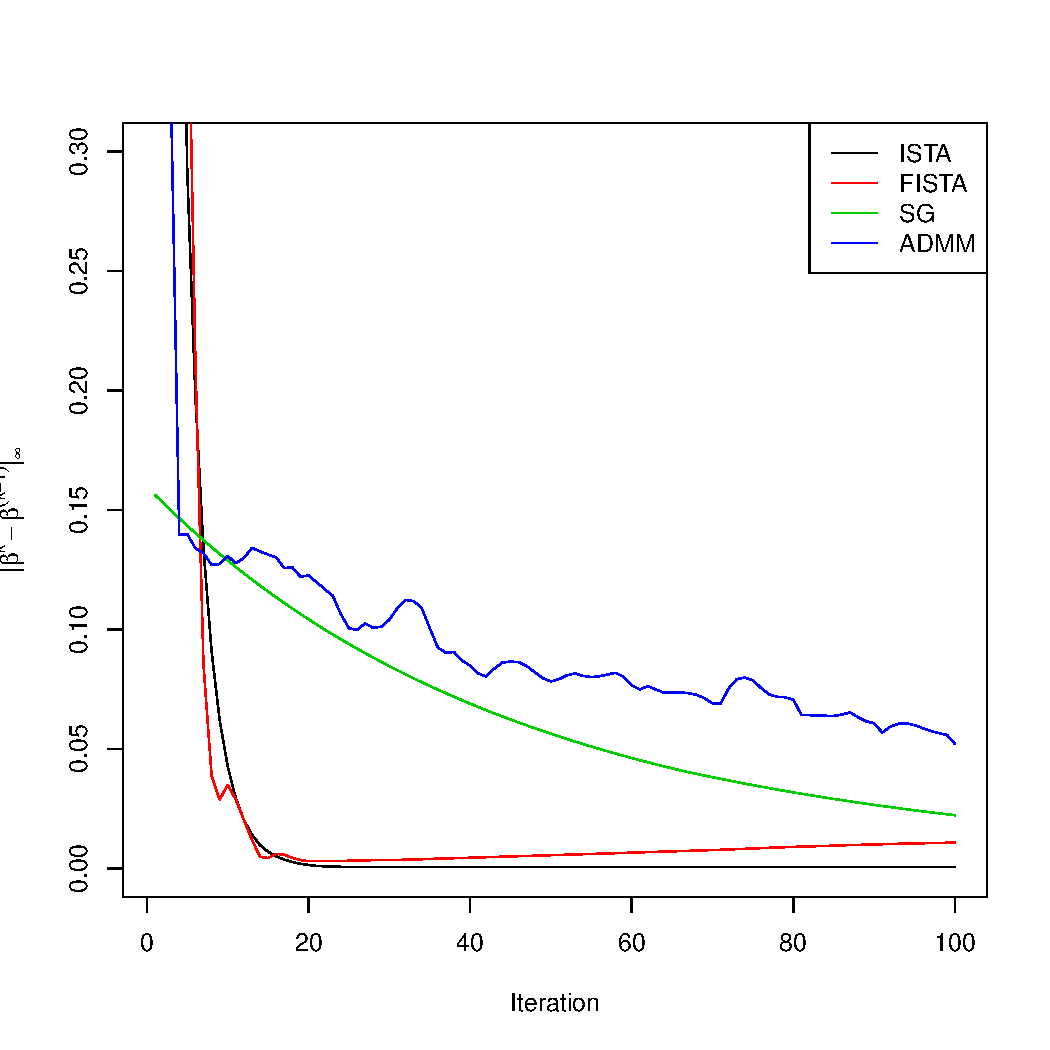
\includegraphics[width=\textwidth]{20cvgc.pdf}
        \caption{$n=20$}
        \label{fig:20}
    \end{subfigure}
~
    \begin{subfigure}[b]{0.4\textwidth}
        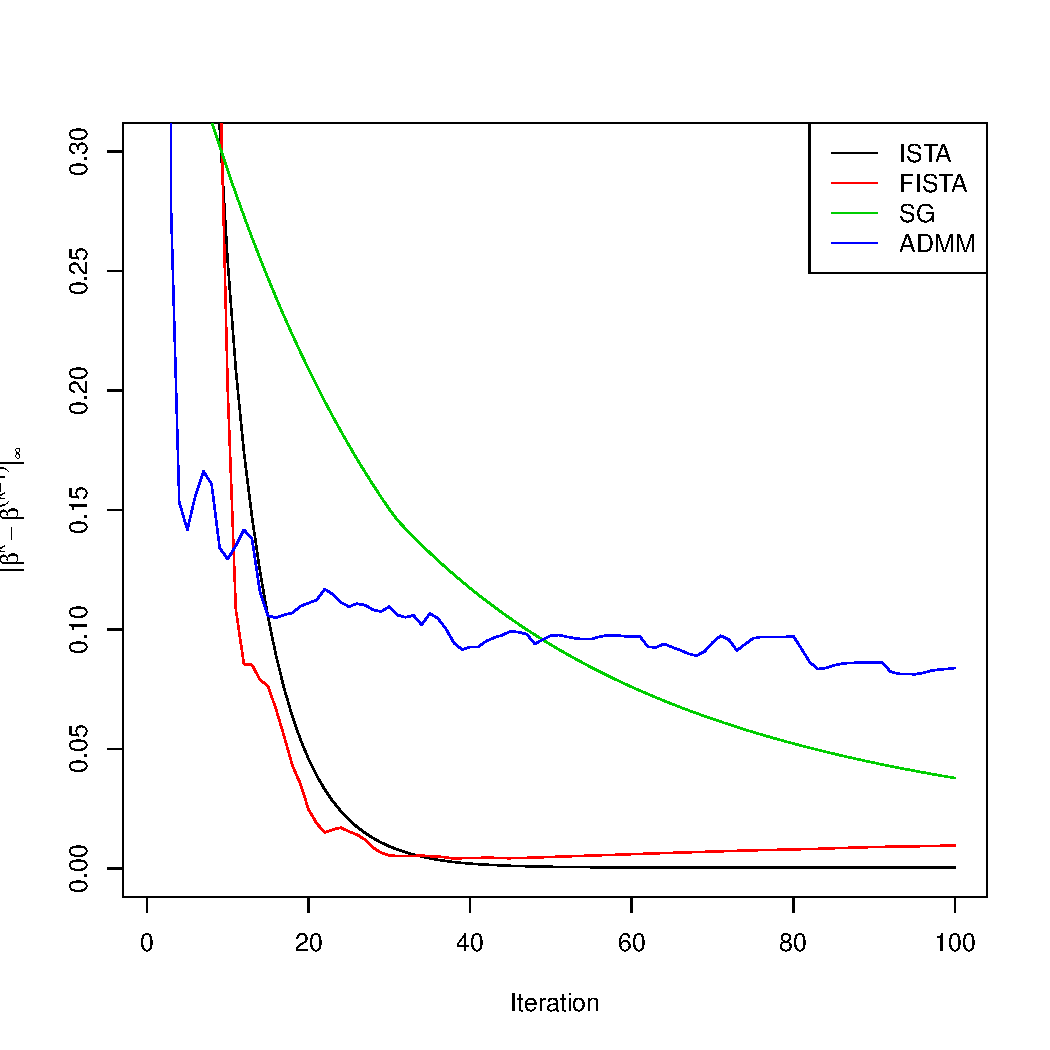
\includegraphics[width=\textwidth]{50cvgc.pdf}
        \caption{$n=50$}
        \label{fig:50}
    \end{subfigure}
\\
    \begin{subfigure}[b]{0.4\textwidth}
        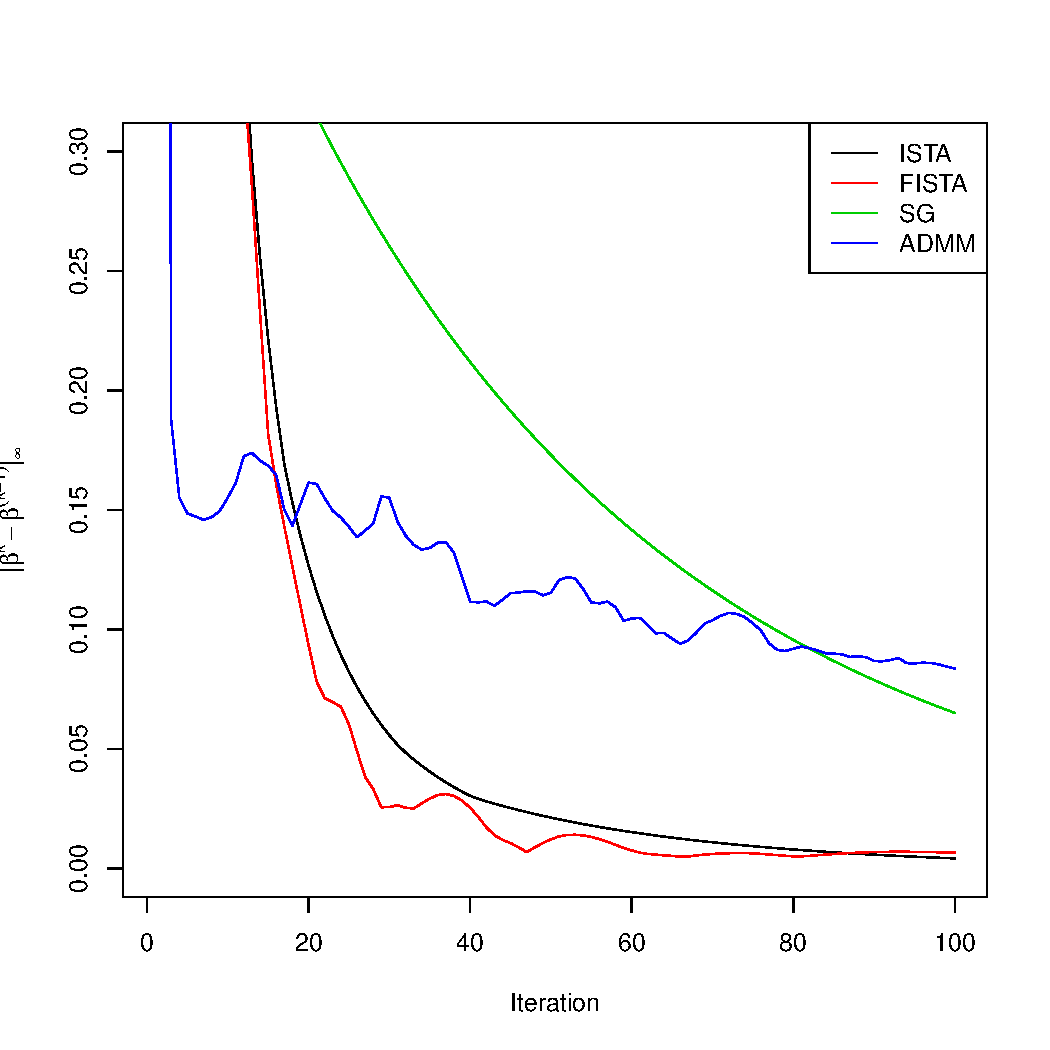
\includegraphics[width=\textwidth]{100cvgc.pdf}
        \caption{$n=100$}
        \label{fig:100}
    \end{subfigure}
~
    \begin{subfigure}[b]{0.4\textwidth}
        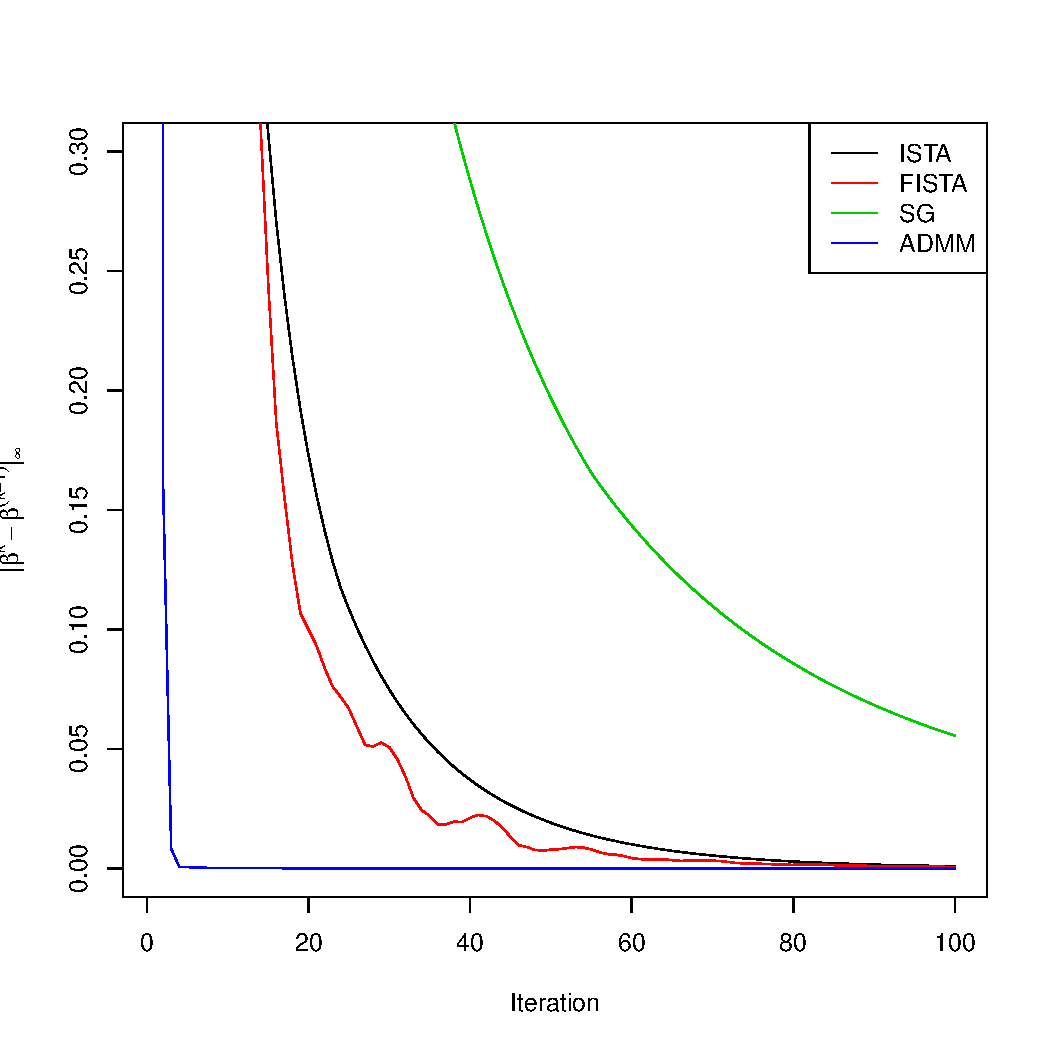
\includegraphics[width=\textwidth]{500cvgc.pdf}
        \caption{$n=500$}
        \label{fig:500}
    \end{subfigure}
\caption{$\norm{\beta^{k}-\beta^{k-1}}_{\infty}$ for the well-conditioned $X$. This checks for convergence of the algorithm. It is clear that according to this measure, ISTA and FISTA perform the best for $n<p$, while ADMM performs the best for the $n>p$ case.}
\label{fig:cvgc}
\end{figure}

\begin{figure}[H]
  \centering
    \begin{subfigure}[b]{0.4\textwidth}
        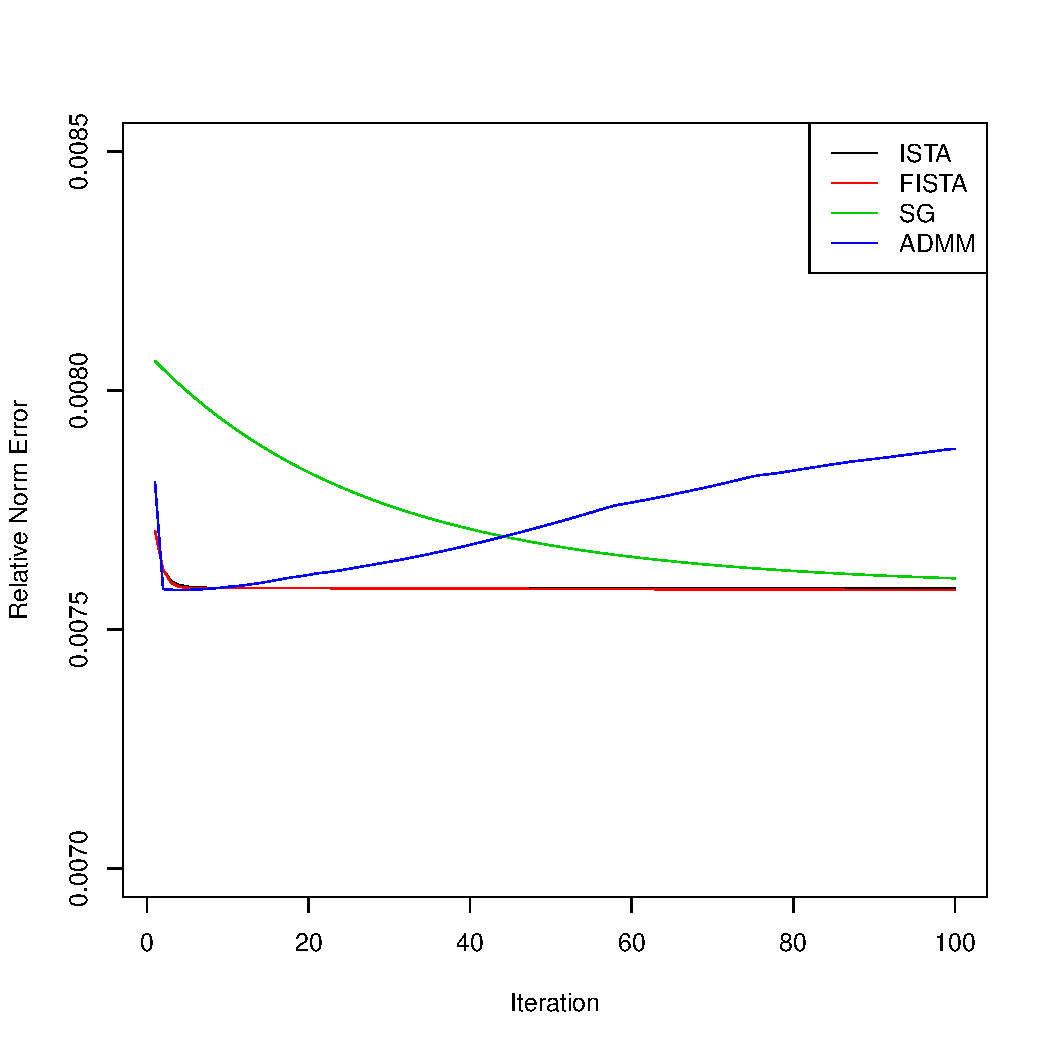
\includegraphics[width=\textwidth]{20cvgc2.pdf}
        \caption{$n=20$}
        \label{fig:20}
    \end{subfigure}
~
    \begin{subfigure}[b]{0.4\textwidth}
        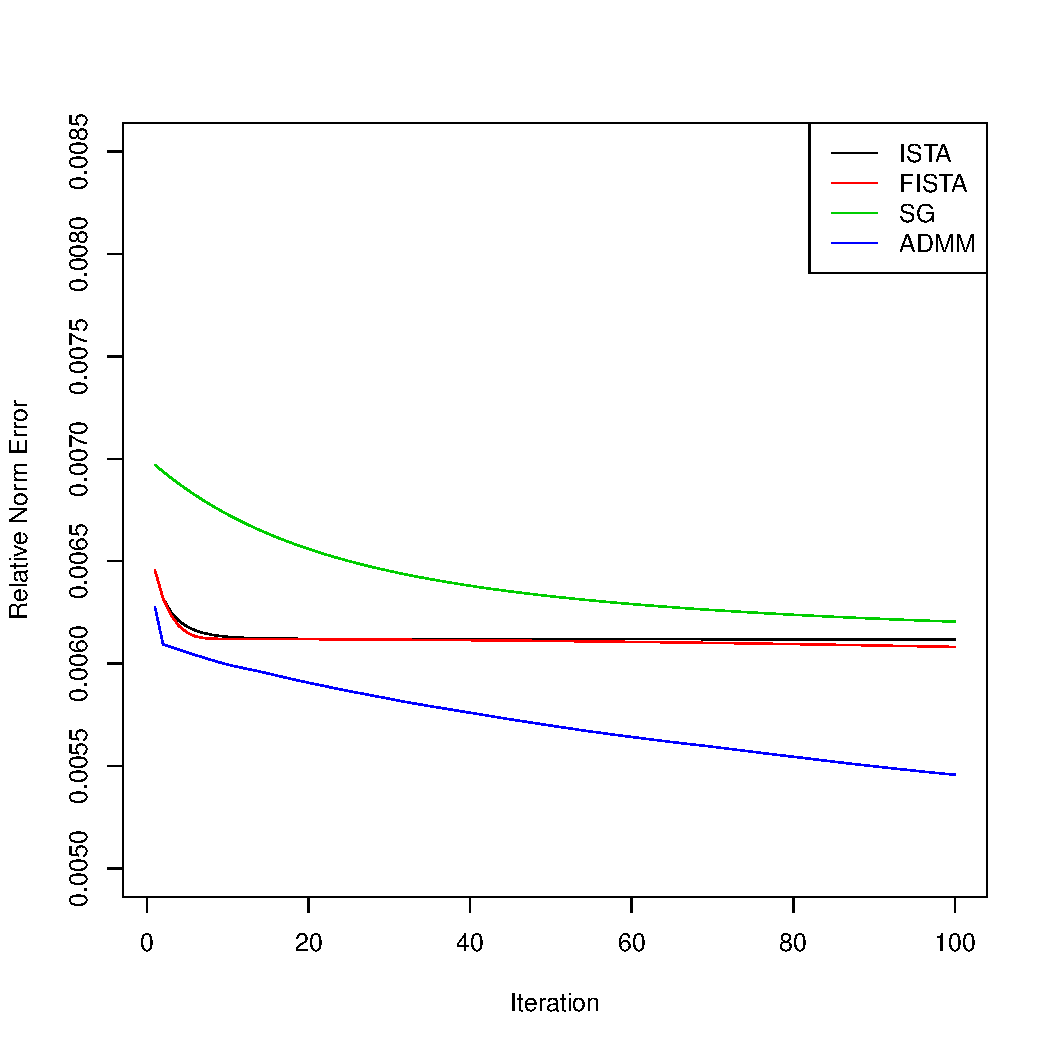
\includegraphics[width=\textwidth]{50cvgc2.pdf}
        \caption{$n=50$}
        \label{fig:50}
    \end{subfigure}
\\
    \begin{subfigure}[b]{0.4\textwidth}
        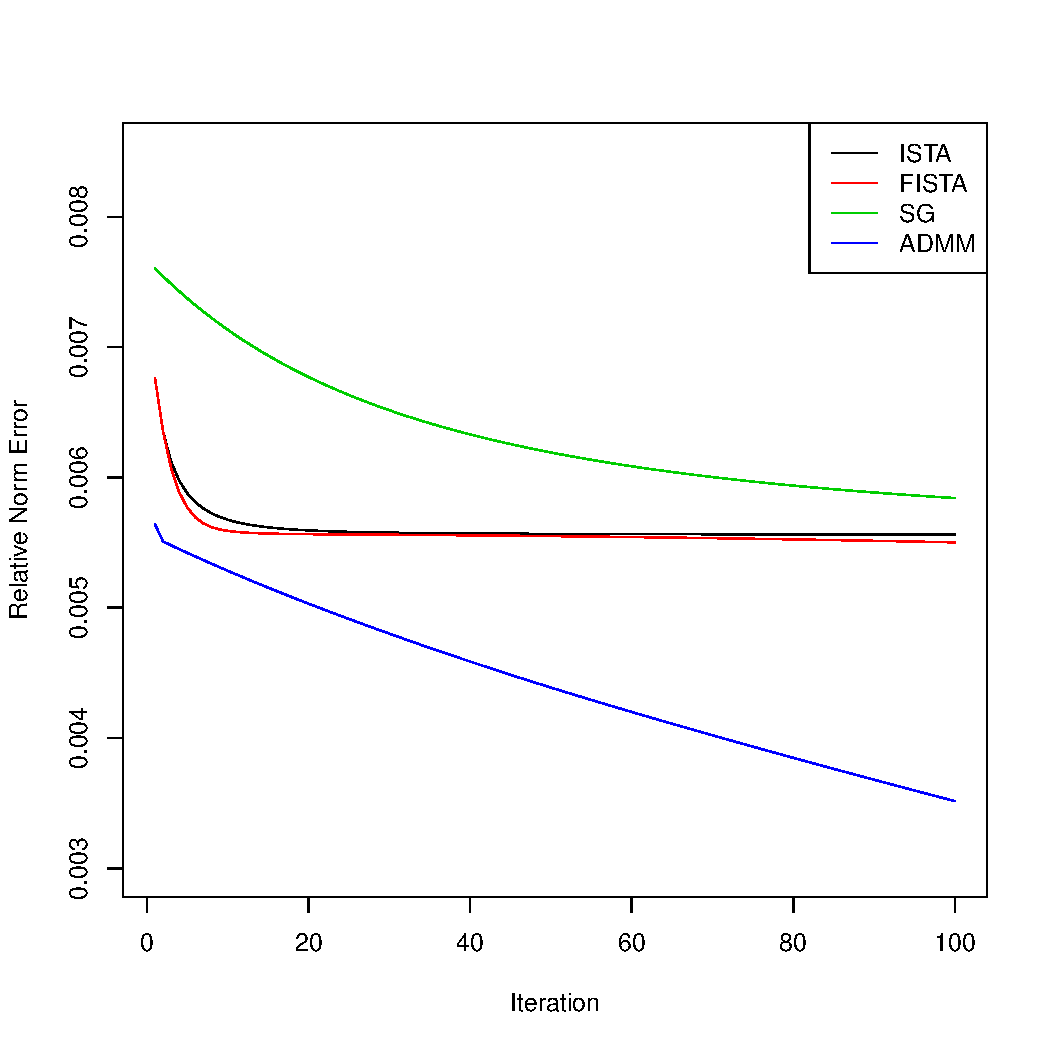
\includegraphics[width=\textwidth]{100cvgc2.pdf}
        \caption{$n=100$}
        \label{fig:100}
    \end{subfigure}
~
    \begin{subfigure}[b]{0.4\textwidth}
        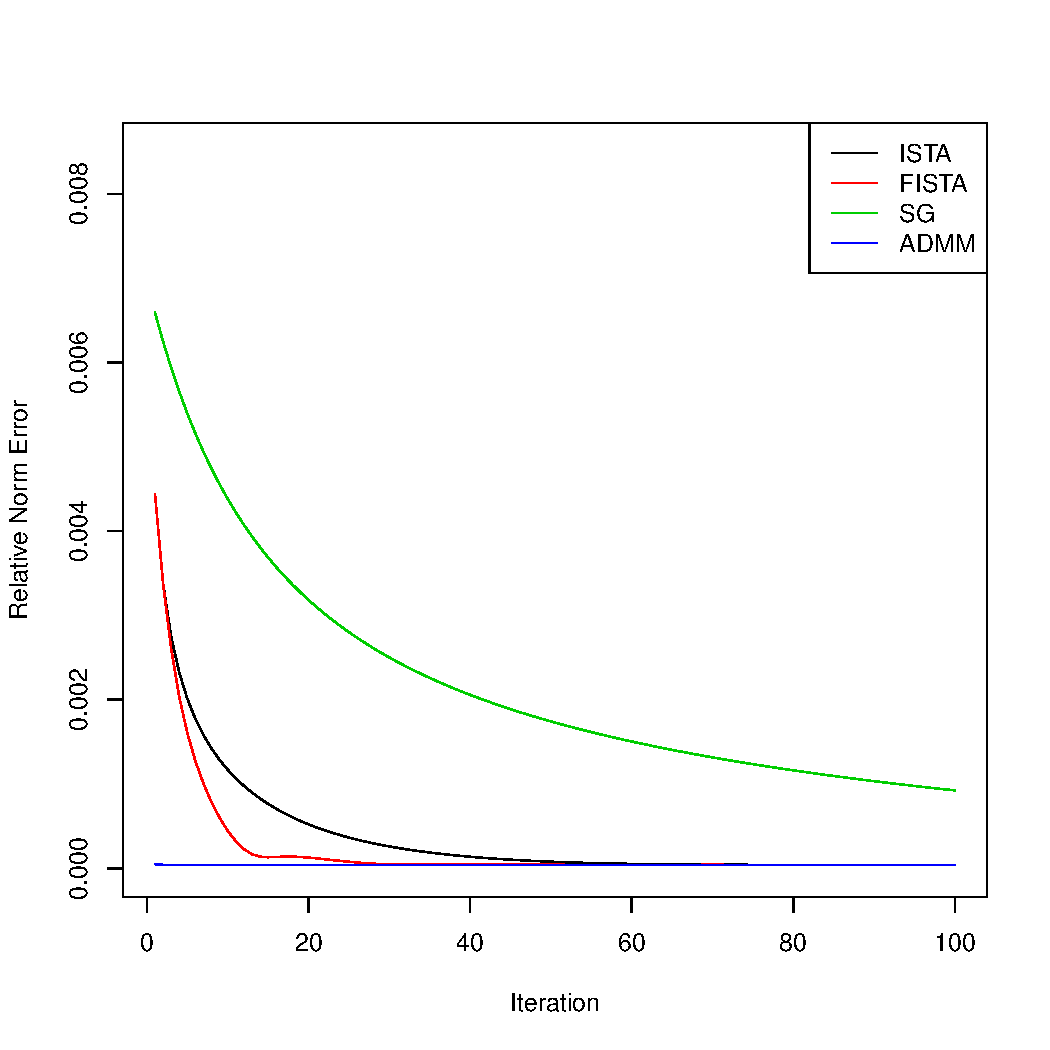
\includegraphics[width=\textwidth]{500cvgc2.pdf}
        \caption{$n=500$}
        \label{fig:500}
    \end{subfigure}
\caption{Relative Normed Error from the true solution for the well conditioned $X$ matrix. This checks for convergence to the true solution. At $n=20$, the performance of ADMM is odd because it starts to rise after initially declining. This is not the case for all the other values of $n$, where it clearly outperforms the other methods.}
\label{fig:cvgc2}
\end{figure}

\begin{figure}[H]
  \centering
    \begin{subfigure}[b]{0.4\textwidth}
        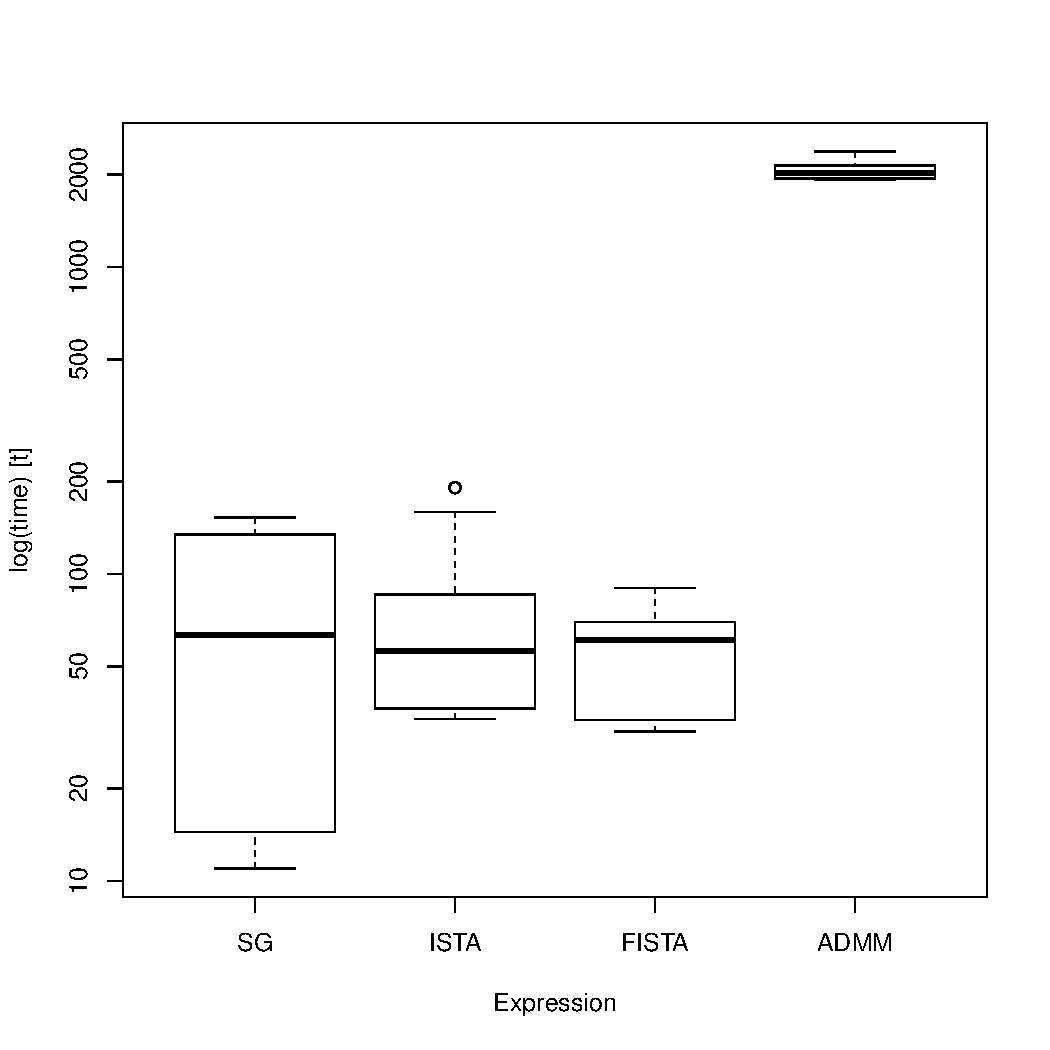
\includegraphics[width=\textwidth]{20timing.pdf}
        \caption{$n=20$}
        \label{fig:20}
    \end{subfigure}
~
    \begin{subfigure}[b]{0.4\textwidth}
        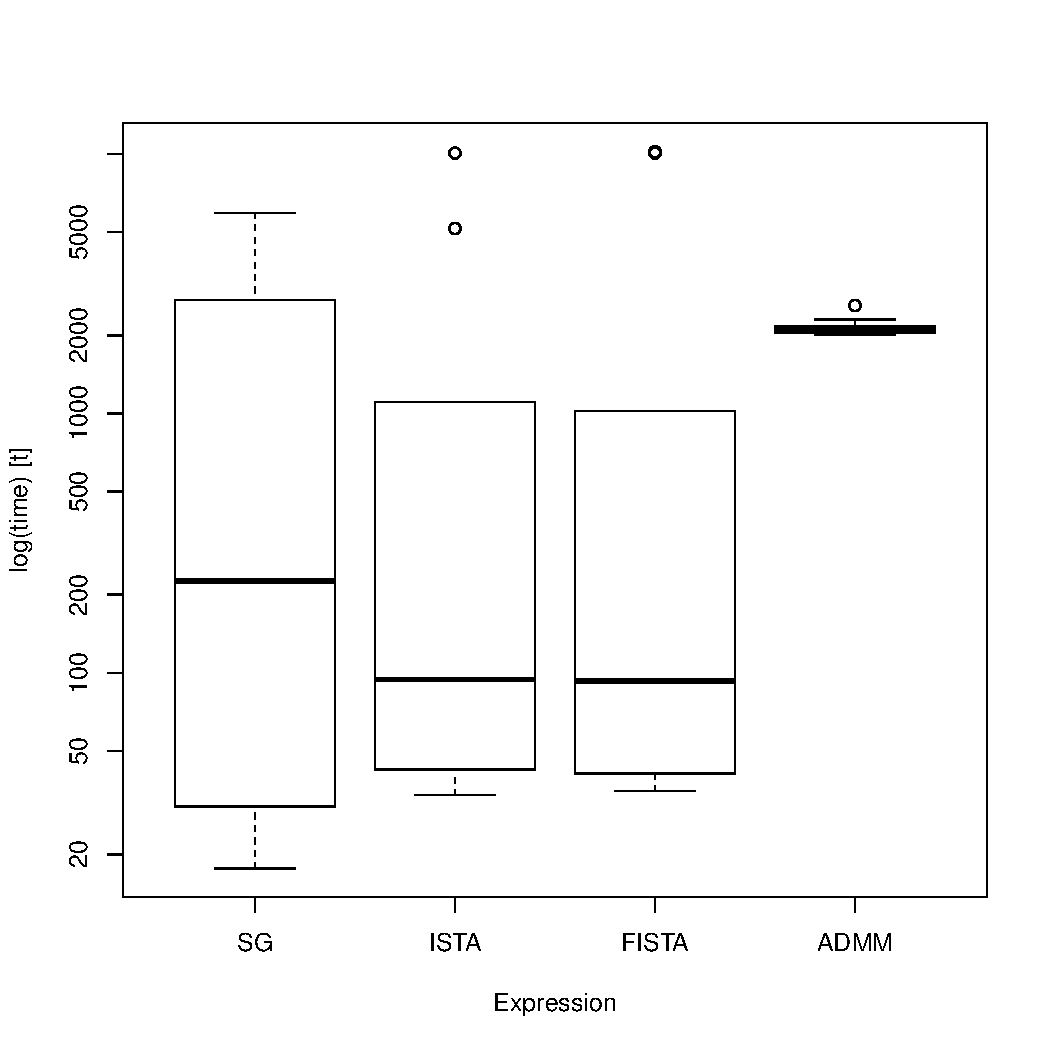
\includegraphics[width=\textwidth]{50timing.pdf}
        \caption{$n=50$}
        \label{fig:50}
    \end{subfigure}
\\
    \begin{subfigure}[b]{0.4\textwidth}
        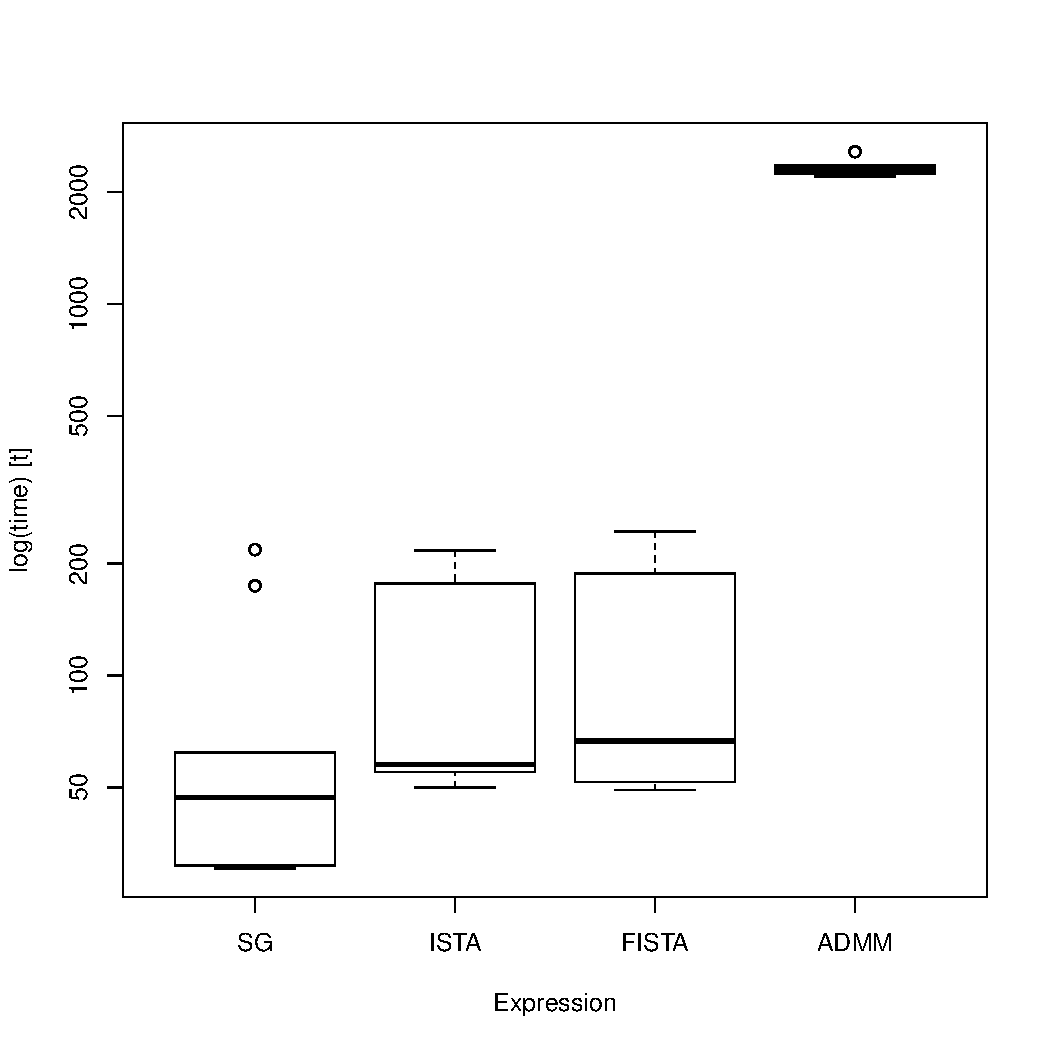
\includegraphics[width=\textwidth]{100timing.pdf}
        \caption{$n=100$}
        \label{fig:100}
    \end{subfigure}
~
    \begin{subfigure}[b]{0.4\textwidth}
        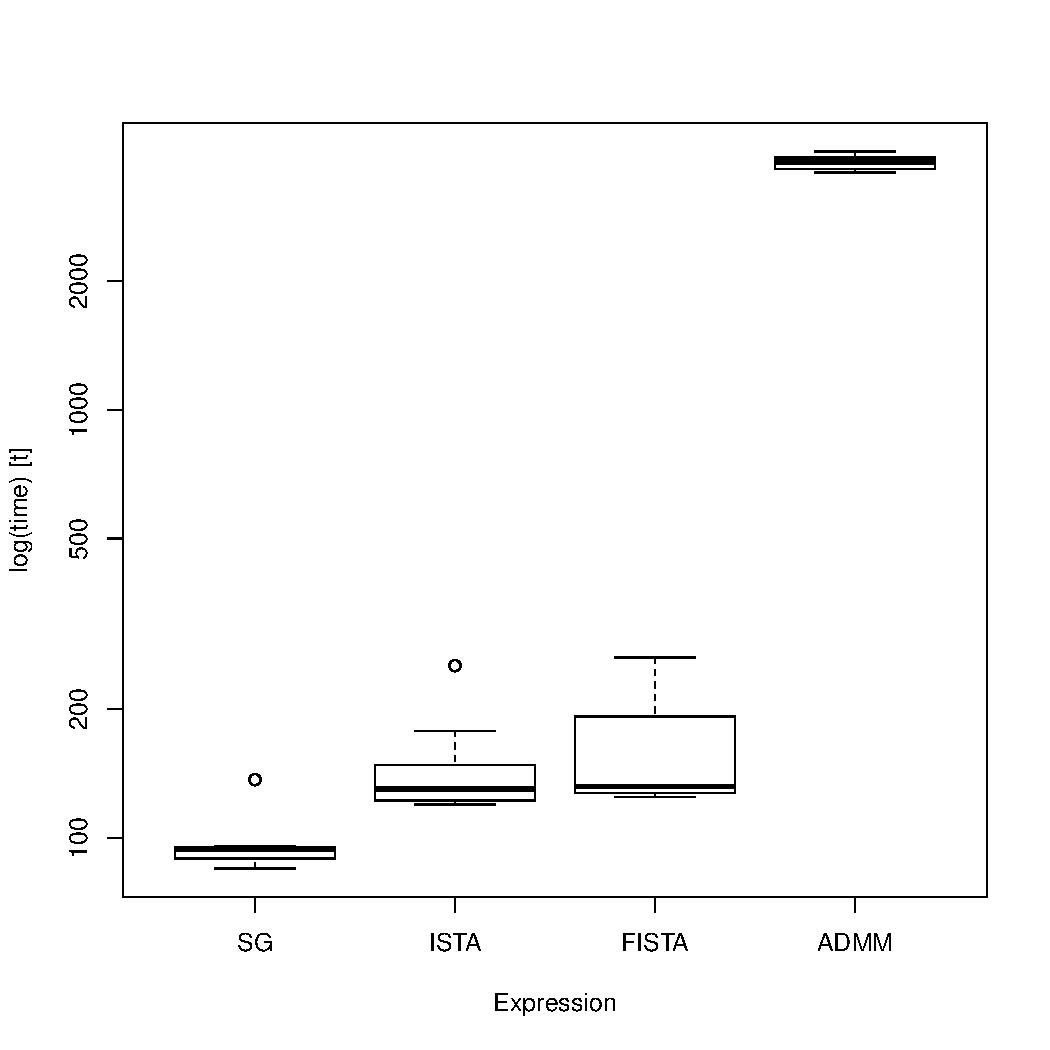
\includegraphics[width=\textwidth]{500timing.pdf}
        \caption{$n=500$}
        \label{fig:500}
    \end{subfigure}
\caption{Timing for Basis Pursuit for well-conditioned $X$. While it is clear that ADMM is the slowesty method, the timing for the other methods is all over the place. Hence it is difficult to find a clear winner in terms of the timing.}
\label{fig:timing}
\end{figure}

\begin{figure}[H]
  \centering
    \begin{subfigure}[b]{0.4\textwidth}
        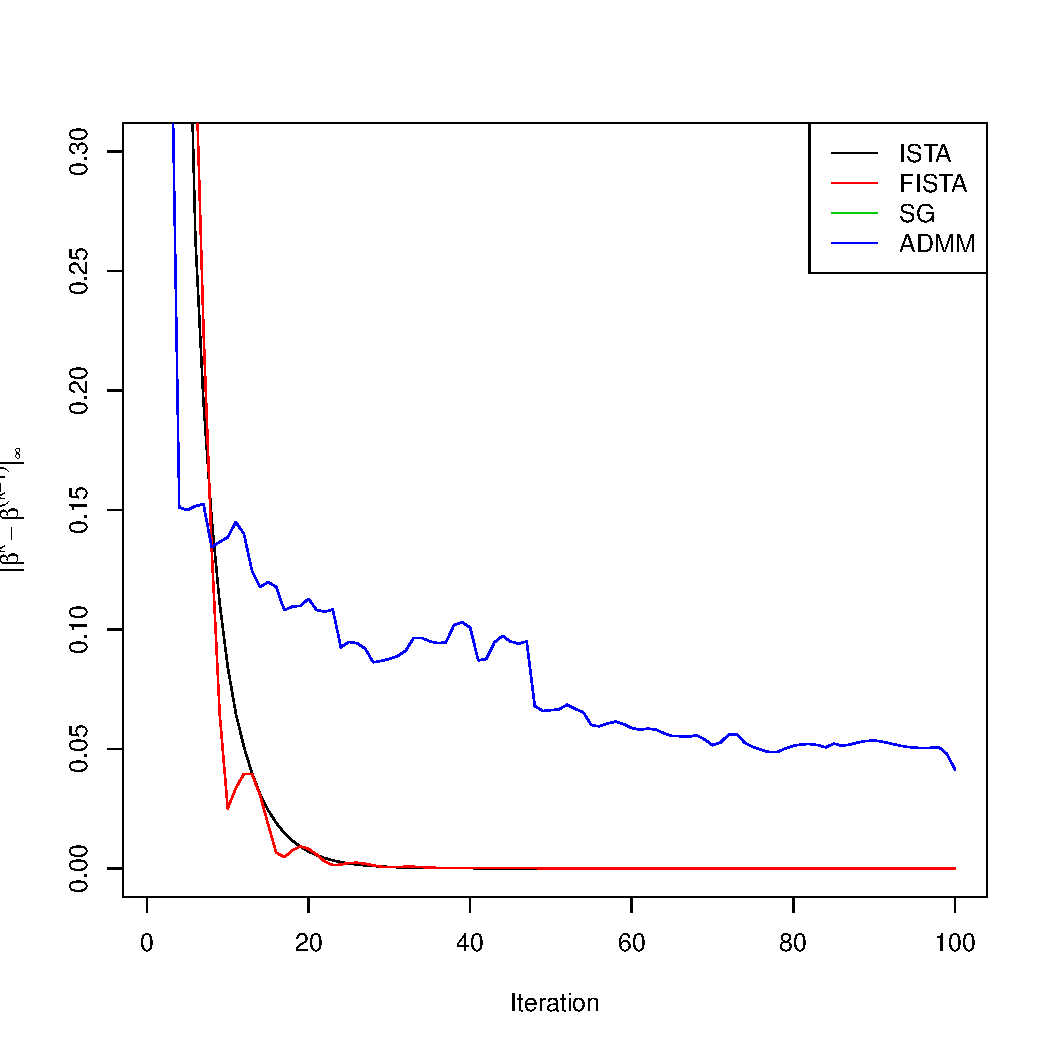
\includegraphics[width=\textwidth]{20cvgc-cn.pdf}
        \caption{$n=20$}
        \label{fig:20}
    \end{subfigure}
~
    \begin{subfigure}[b]{0.4\textwidth}
        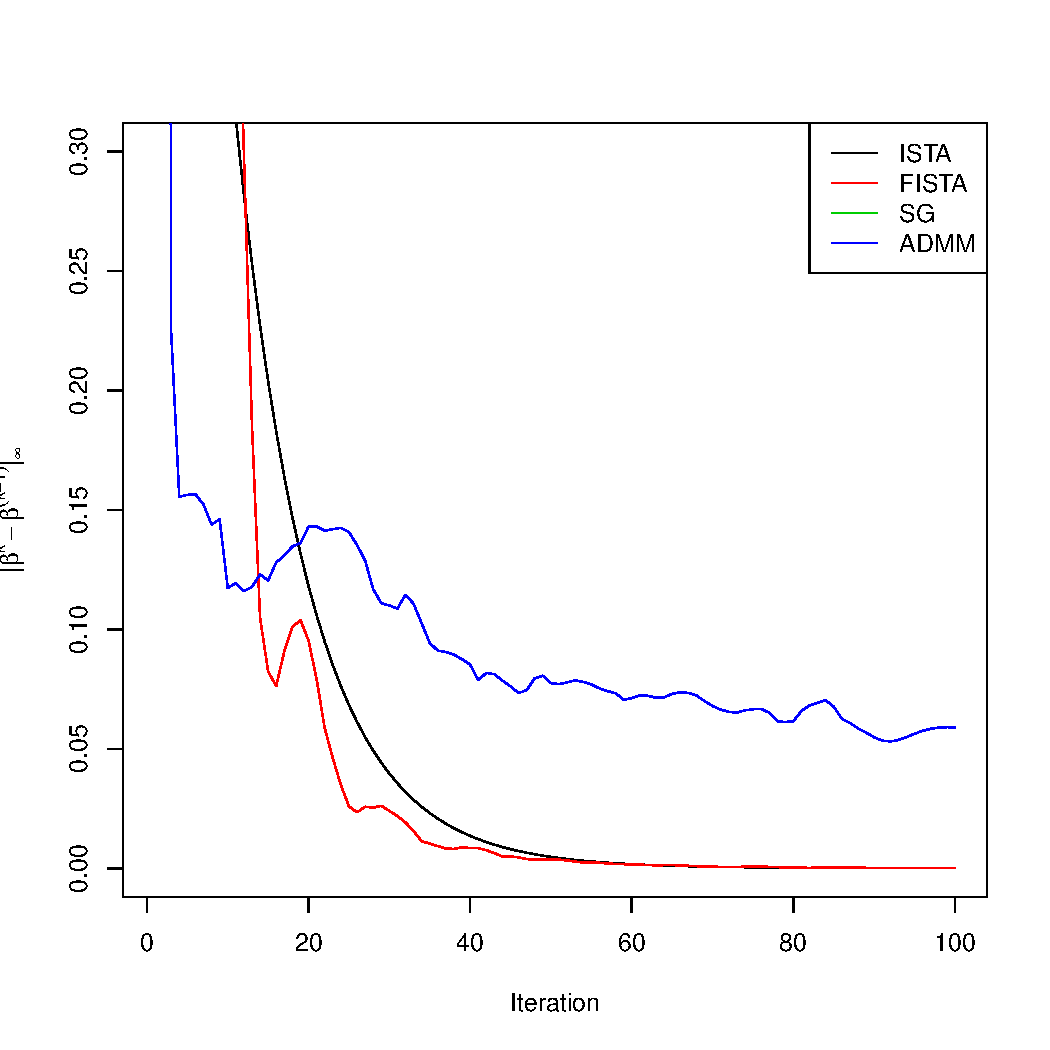
\includegraphics[width=\textwidth]{50cvgc-cn.pdf}
        \caption{$n=50$}
        \label{fig:50}
    \end{subfigure}
\\
    \begin{subfigure}[b]{0.4\textwidth}
        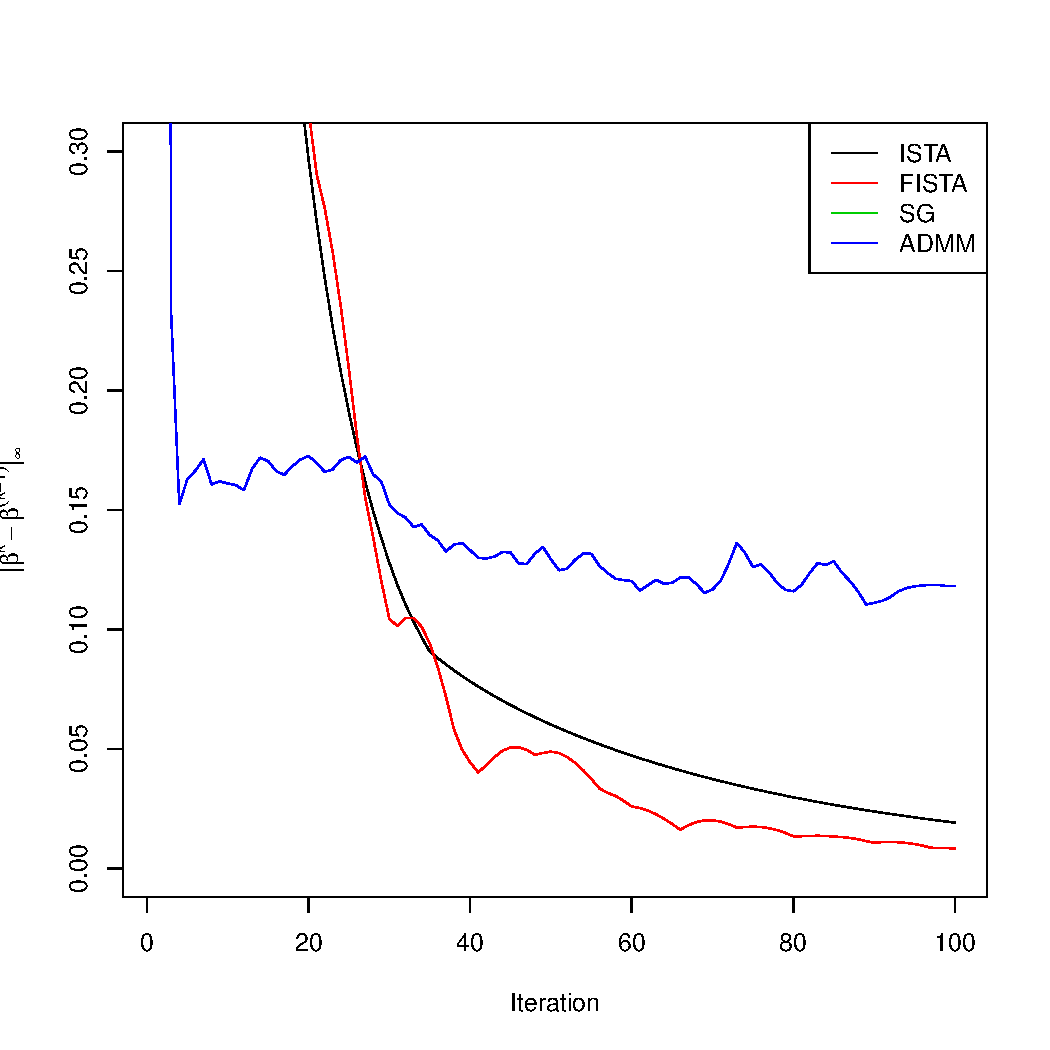
\includegraphics[width=\textwidth]{100cvgc-cn.pdf}
        \caption{$n=100$}
        \label{fig:100}
    \end{subfigure}
~
    \begin{subfigure}[b]{0.4\textwidth}
        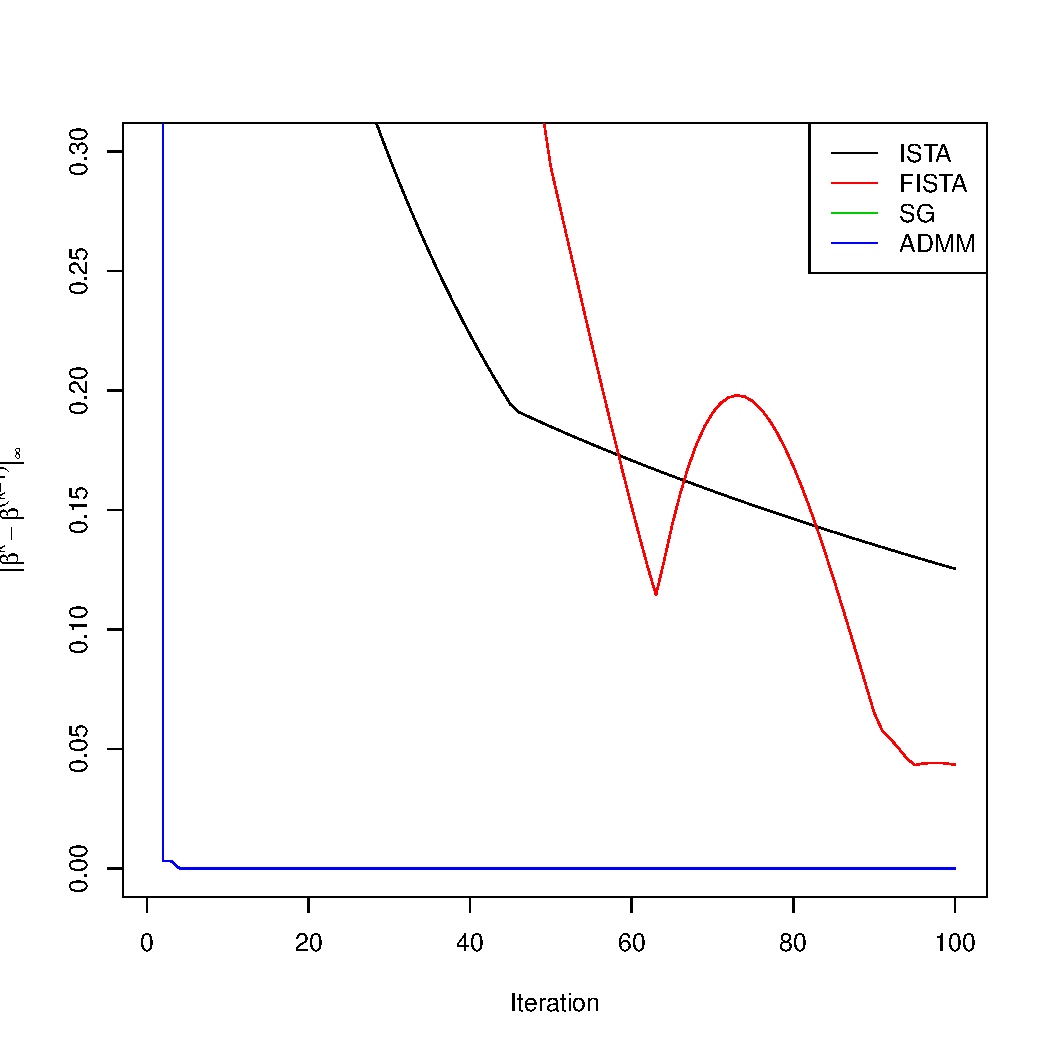
\includegraphics[width=\textwidth]{500cvgc-cn.pdf}
        \caption{$n=500$}
        \label{fig:500}
    \end{subfigure}
\caption{$\norm{\beta^{k}-\beta^{k-1}}_{\infty}$ for the ill-conditioned $X$. This checks for convergence of the algorithm. The sub-gradient algorithm diverges in this case and hence doesn't appear on the plots. It is clear that according to this measure, ISTA and FISTA performs erratically, but is still the best for $n<p$, while ADMM performs the best for the $n>p$ case.}
\label{fig:cvgccn}
\end{figure}

\begin{figure}[H]
  \centering
    \begin{subfigure}[b]{0.4\textwidth}
        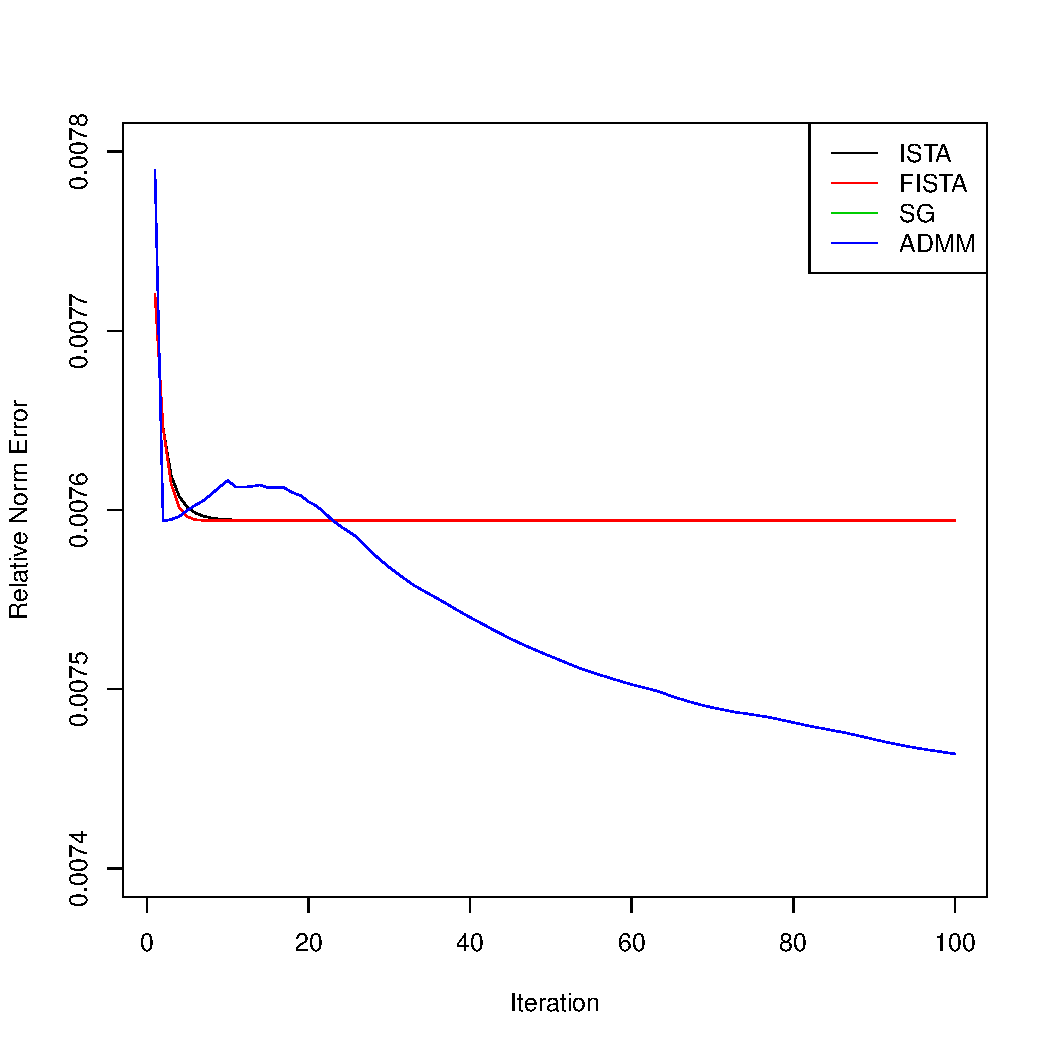
\includegraphics[width=\textwidth]{20cvgc2-cn.pdf}
        \caption{$n=20$}
        \label{fig:20}
    \end{subfigure}
~
    \begin{subfigure}[b]{0.4\textwidth}
        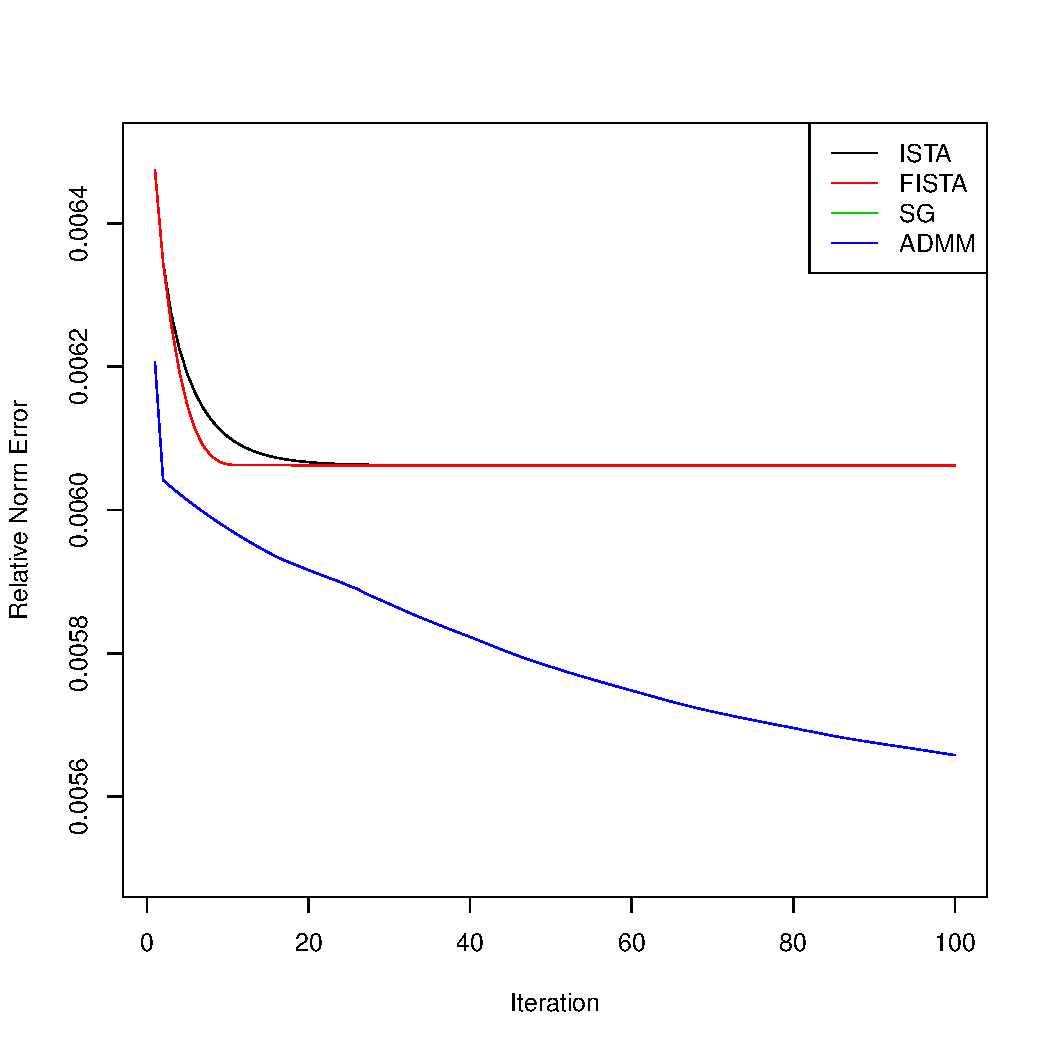
\includegraphics[width=\textwidth]{50cvgc2-cn.pdf}
        \caption{$n=50$}
        \label{fig:50}
    \end{subfigure}
\\
    \begin{subfigure}[b]{0.4\textwidth}
        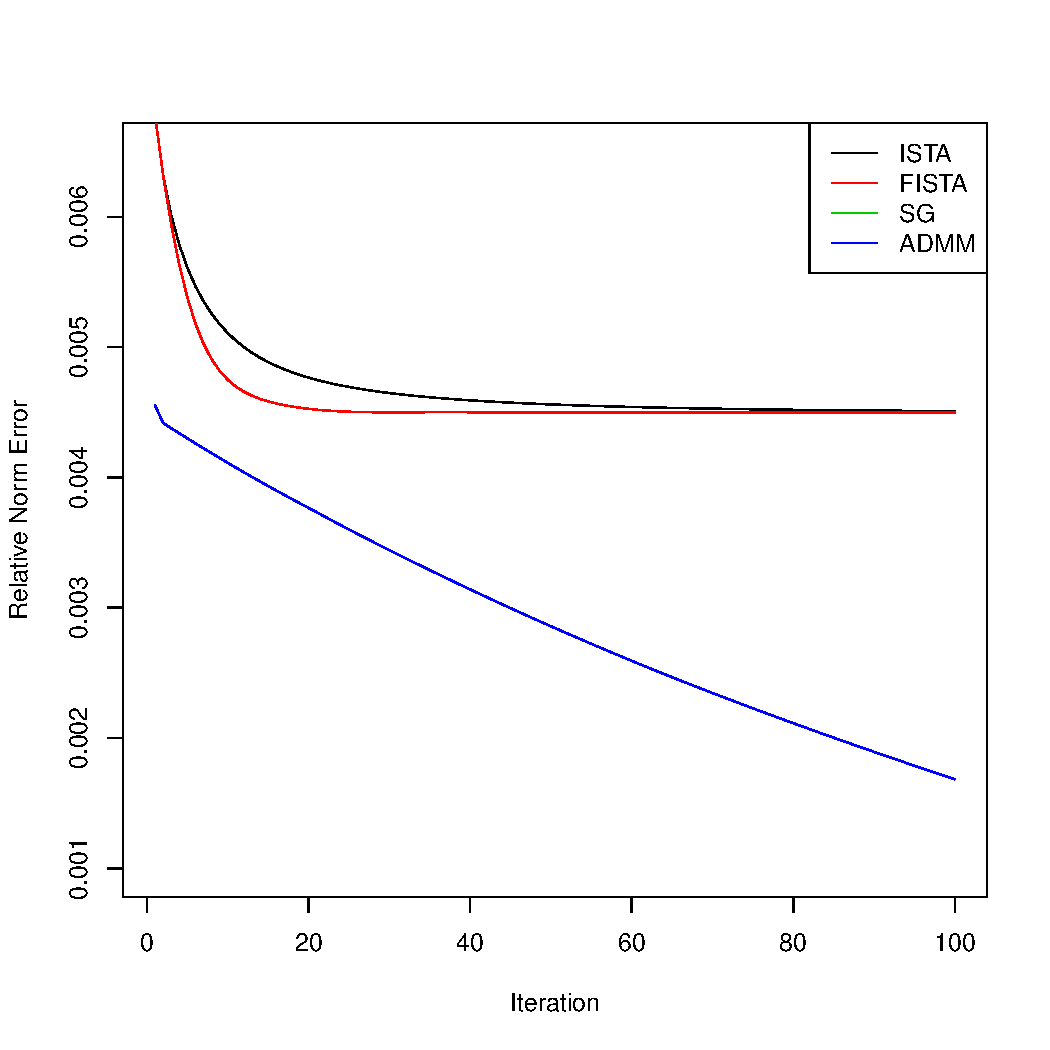
\includegraphics[width=\textwidth]{100cvgc2-cn.pdf}
        \caption{$n=100$}
        \label{fig:100}
    \end{subfigure}
~
    \begin{subfigure}[b]{0.4\textwidth}
        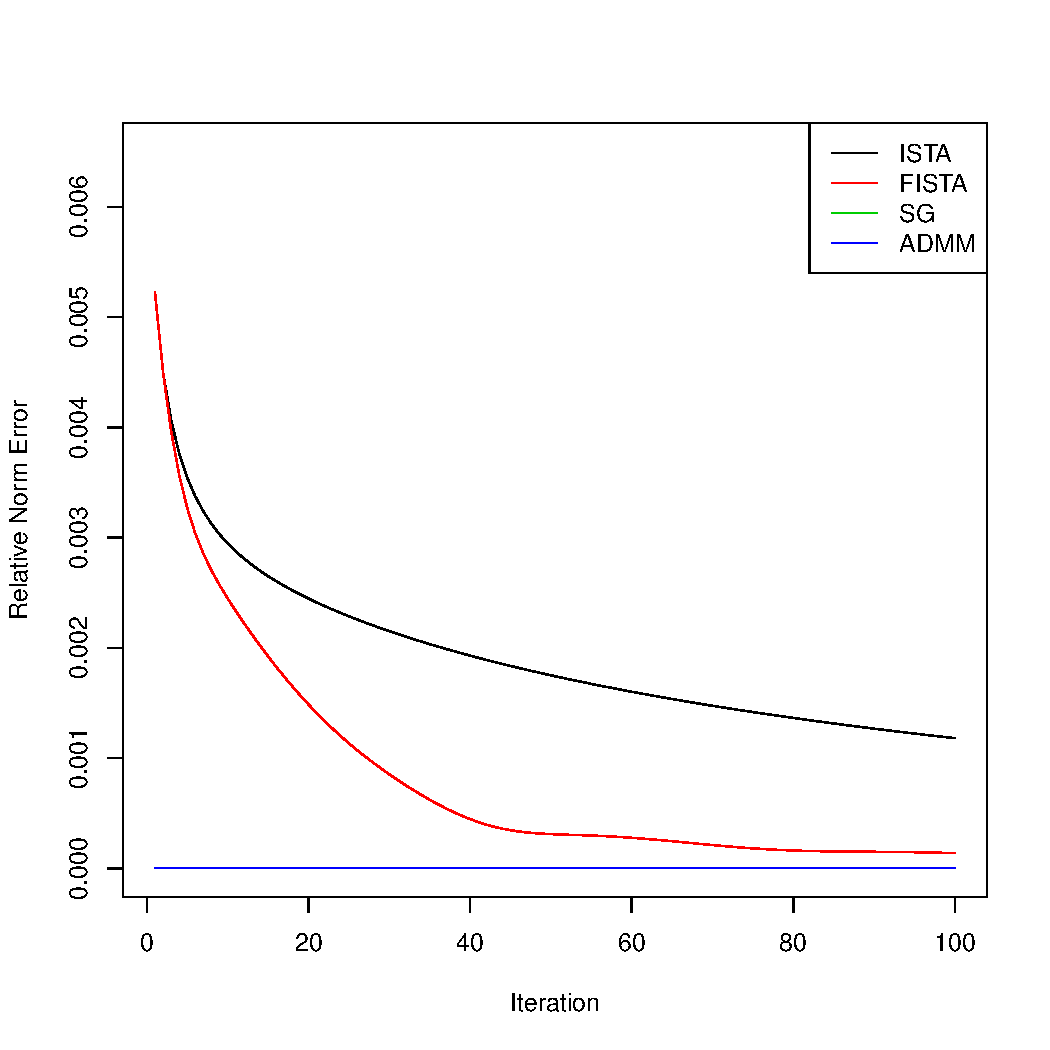
\includegraphics[width=\textwidth]{500cvgc2-cn.pdf}
        \caption{$n=500$}
        \label{fig:500}
    \end{subfigure}
\caption{Relative Normed Error from the true solution for the ill-conditioned $X$ matrix. This checks for convergence to the true solution. ADMM clearly performs the best in this case.}
\label{fig:cvgc2cn}
\end{figure}

\begin{figure}[H]
  \centering
    \begin{subfigure}[b]{0.4\textwidth}
        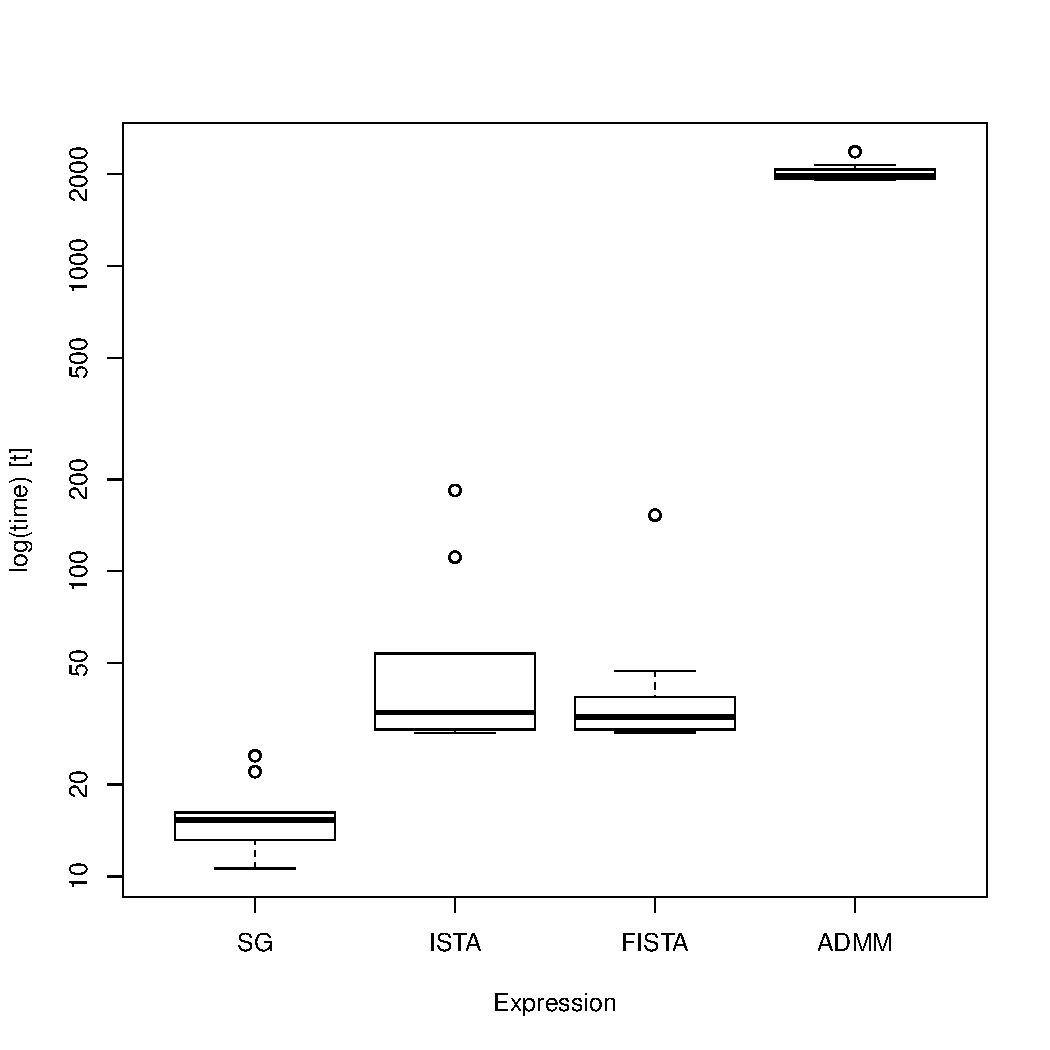
\includegraphics[width=\textwidth]{20timing-cn.pdf}
        \caption{$n=20$}
        \label{fig:20}
    \end{subfigure}
~
    \begin{subfigure}[b]{0.4\textwidth}
        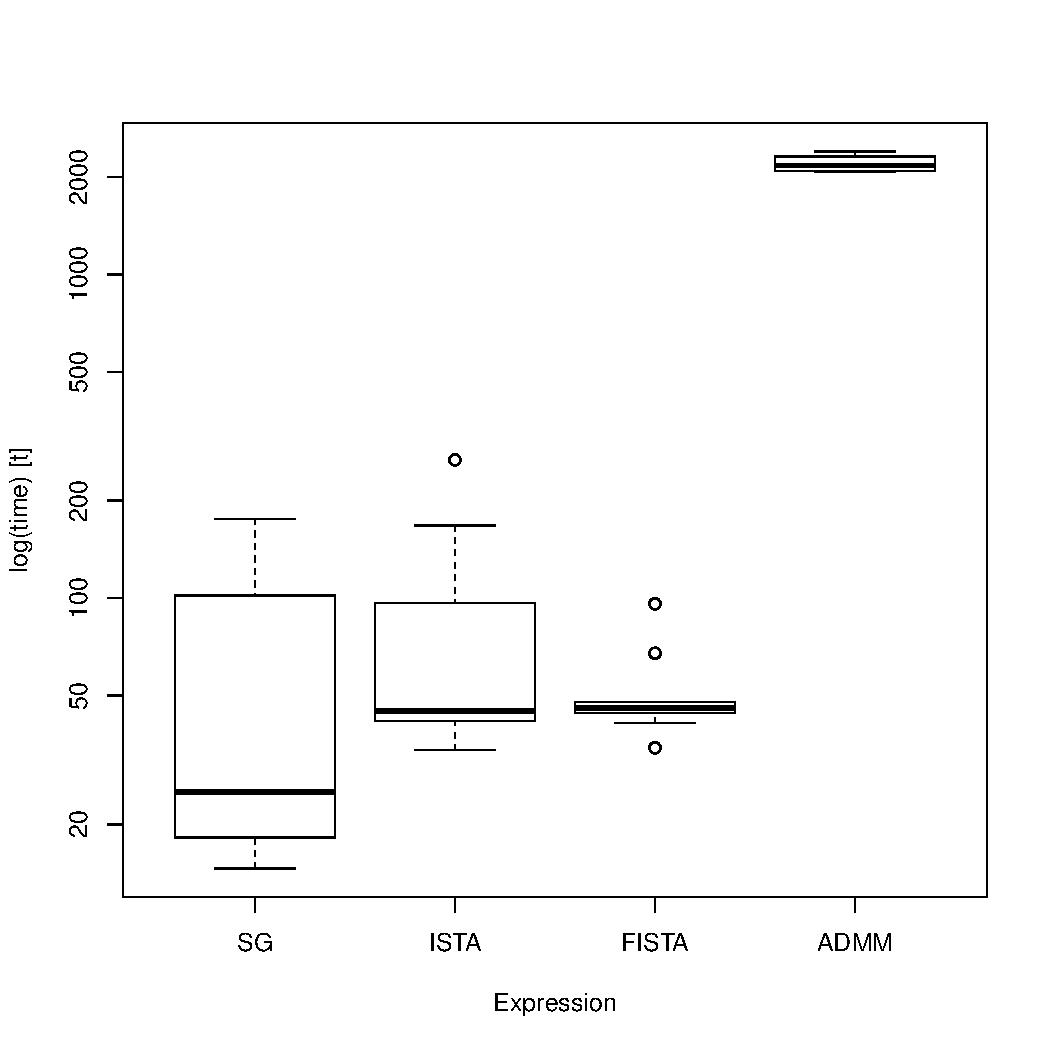
\includegraphics[width=\textwidth]{50timing-cn.pdf}
        \caption{$n=50$}
        \label{fig:50}
    \end{subfigure}
\\
    \begin{subfigure}[b]{0.4\textwidth}
        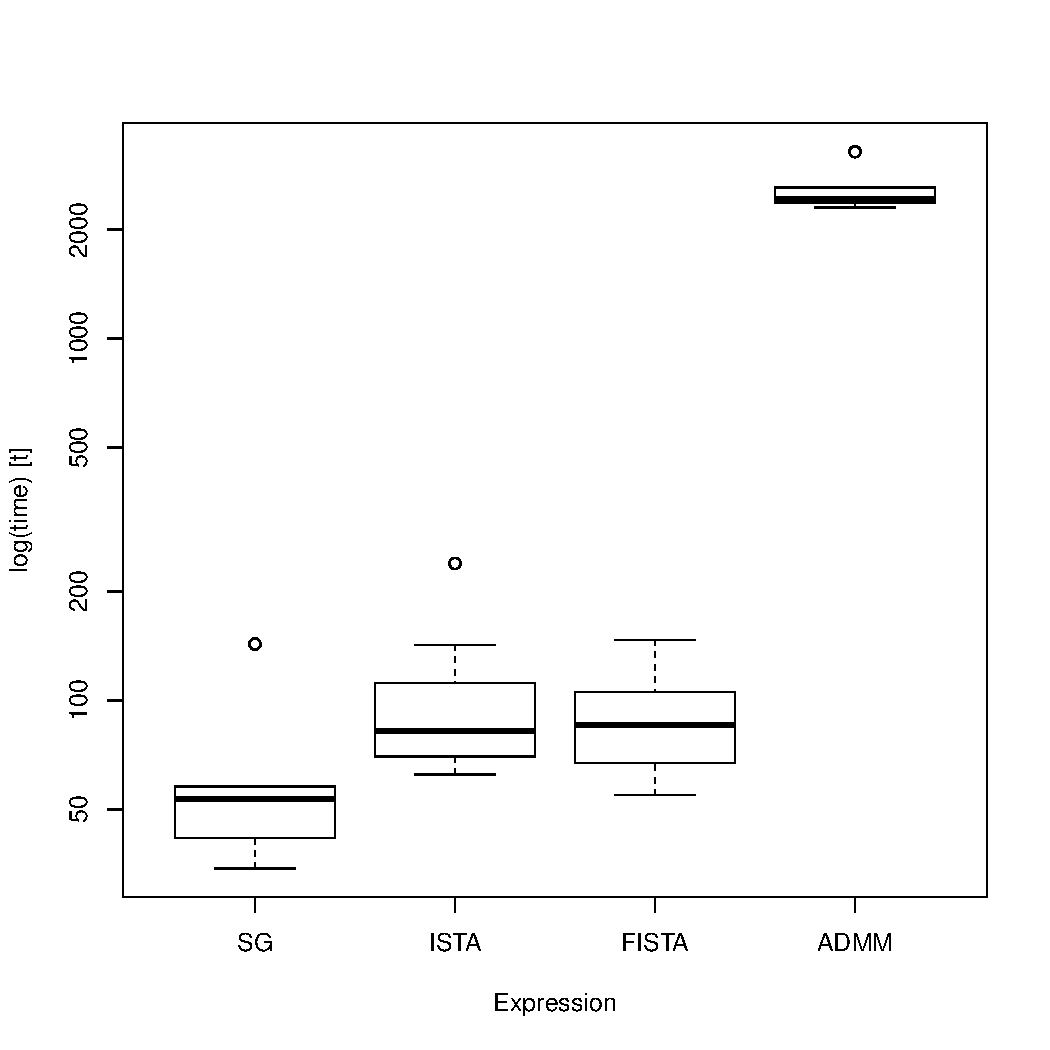
\includegraphics[width=\textwidth]{100timing-cn.pdf}
        \caption{$n=100$}
        \label{fig:100}
    \end{subfigure}
~
    \begin{subfigure}[b]{0.4\textwidth}
        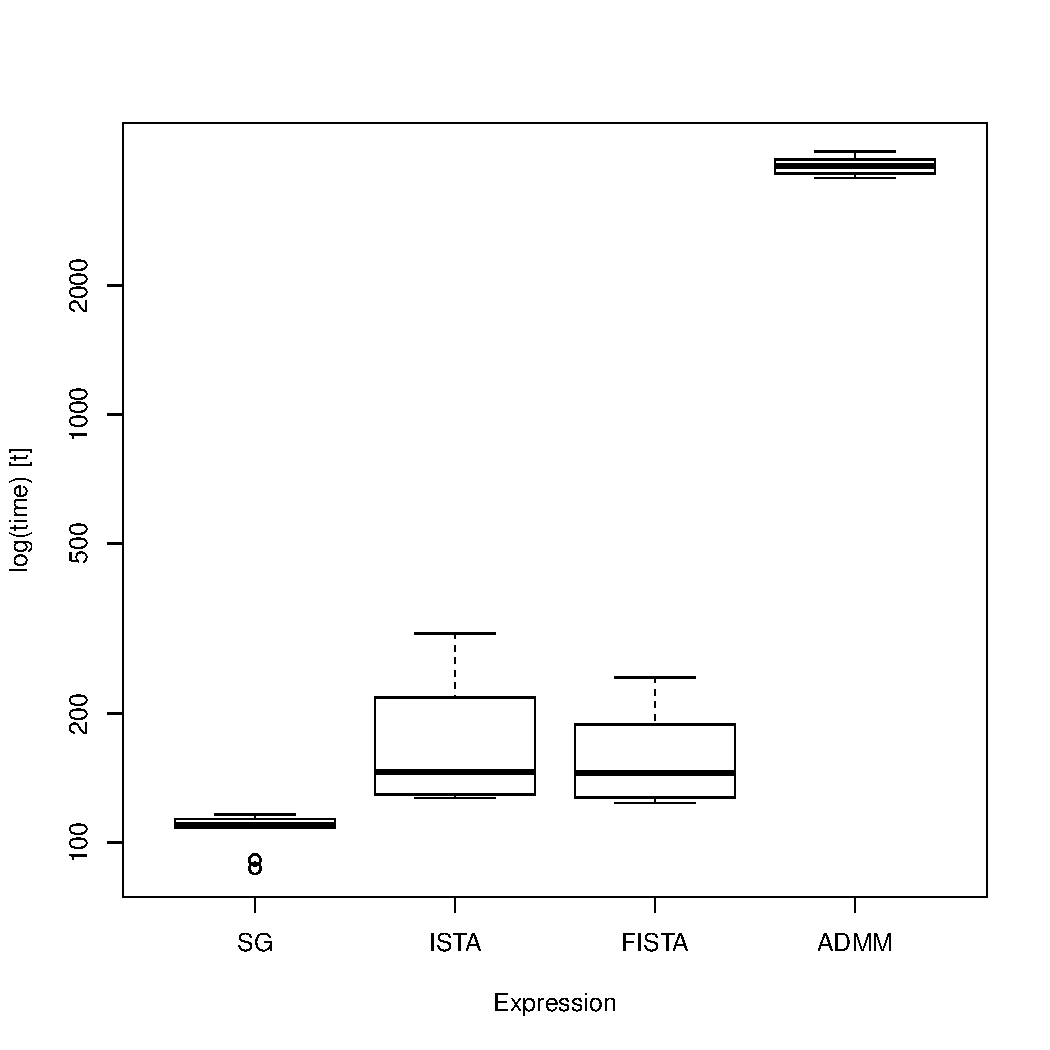
\includegraphics[width=\textwidth]{500timing-cn.pdf}
        \caption{$n=500$}
        \label{fig:500}
    \end{subfigure}
\caption{Timing for Basis Pursuit for ill-conditioned $X$. It is clear that ADMM is the slowesty method with the other methods performing much better. However, in terms of the other measures, their performance was poorer as compared to the ADMM.}
\label{fig:timingcn}
\end{figure}

\pagebreak

\begin{thebibliography}{Tototo}
\bibitem{Beck} Beck, A. and Teboulle, M. (2009), {``A Fast Iterative Shrinkage-Thresholding Algorithm
for Linear Inverse Problems}, \emph{Siam J. Imaging Sciences} Vol. 2, No. 1, pp. 183-202
\bibitem{Boyd2011} Boyd, S. and Parikh, N. and Chu, E. and Peleato, B.  (2011), {``Distributed Optimization and Statistical Learning via the Alternating Direction Method of Multipliers,''} \emph{Foundations and Trends in
Machine Learning}, Vol. 3, No. 1, 1-122
\bibitem{Boyd}  Boyd, S. and Vandenberghe, L. (2009), {``Convex Optimization,''} 
\end{thebibliography}

\end{document}